\باب{وقت کے ساتھ بدلتے میدان اور میکس ویل کے مساوات}\شناخت{باب_میکس_ویل}
گزشتہ بابوں میں وقت کے ساتھ تبدیل نہ ہونے والے میدانوں پر غور کیا گیا۔بقایا کتاب میں وقت کے ساتھ تبدیل ہوتے میدانوں پر غور کیا جائے گا۔

اس باب میں دو نئے اصولوں پر غور کیا جائے گا۔پہلا اصول مائکل فیراڈے نے تجرباتی طور پر ثابت کیا جس کے تحت وقت کے ساتھ بدلتا مقناطیسی میدان، برقی میدان کو جنم دیتا ہے۔دوسرا قانون  جیمس کلارک میکس ویل کے کاوشوں سے حاصل ہوا جس کے تحت وقت کے ساتھ بدلتا برقی میدان، مقناطیسی میدان کو جنم دیتا ہے۔ اس باب میں برقی و مقناطیسیات کے چار ایسے مساوات پیش کئے جائیں گے جو \اصطلاح{میکس ویل مساوات}\فرہنگ{میکس ویل مساوات} کہلاتے ہیں۔

\حصہ{فیراڈے کا قانون}
جناب مائکل فیراڈے نے تجرباتی طور پر ثابت کیا کہ وقت کے ساتھ بدلتا مقناطیسی میدان، برقی میدان پیدا کرتا ہے۔\اصطلاح{قانون فیراڈے}\فرہنگ{قانون!فیراڈے}\فرہنگ{فیراڈے!قانون}\حاشیہب{Faraday's law}\فرہنگ{Faraday's law} کو مندرجہ ذیل مساوات پیش کرتی ہے۔
\begin{align}\label{مساوات_میکس_ویل_فیراڈے_قانون}
\textrm{\RL{محرک برقی دباو}}=-\frac{\dif \Phi}{\dif t}
\end{align}
اس قانون کے تحت کسی بھی سطح سے گزرتی مقناطیسی بہاو کی قیمت میں تبدیلی،  اس سطح کے محیط پر برقی دباو پیدا کرتی ہے۔ایسی برقی دباو روایتی طور پر \اصطلاح{محرک برقی دباو}\فرہنگ{محرک برقی دباو}\حاشیہب{electromotive force, emf}\فرہنگ{electromotive force}\فرہنگ{emf} کہلاتی ہے۔کسی بھی سطح کے محیط پر محرک برقی دباو\حاشیہد{محرک برقی دباو کی اصطلاح روایتی طور پر ہر قسم کے منبع برقی دباو کے لئے استعمال کی جاتی ہے۔} کی قیمت، اس سطح سے گزرتی مقناطیسی بہاو کے قیمت میں تبدیلی کی شرح کے برابر ہوتی ہے۔محرک برقی دباو کی اکائی وولٹ \عددیء{\si{\volt}} ہے۔سطح کے محیط کو بند دائرہ تصور کرتے ہوئے ہم یوں بھی کہہ سکتے ہیں کہ کسی بھی بند دائرے پر محرک برقی دباو کی قیمت اس دائرے  کے اندر سے گزرتی مقناطیسی بہاو کے قیمت میں تبدیلی کی شرح کے برابر ہو گی۔یہاں یہ سمجھ لینا ضروری ہے کہ بند دائرہ فرضی لکیر بھی ہو سکتا ہے۔
 
ابتدائی مقناطیسی بہاو میں تبدیلی، محرک برقی دباو پیدا کرتی ہے۔محرک برقی دباو مکمل برقی دور میں برقی رو پیدا کرنے کی صلاحیت رکھتا ہے۔محرک برقی دباو سے پیدا برقی رو، بند دائرے میں ثانوی مقناطیسی بہاو پیدا کرے گی۔ثانوی مقناطیسی بہاو،  ابتدائی مقناطیسی بہاو میں تبدیلی کو روکنے کی کوشش کرتی ہے۔مساوات \حوالہ{مساوات_میکس_ویل_فیراڈے_قانون} میں منفی کی علامت اسی اصول کو بیان کرتی ہے، یعنی کہ، بند دائرے میں محرک برقی دباو سے پیدا برقی رو، پہلے سے موجود مقناطیسی بہاو میں تبدیلی کو روکنے کی کوشش کرتی ہے۔یہ اصول \اصطلاح{لینز}\فرہنگ{قانون!لینز}\حاشیہد{یہ قانون 1834 میں جناب لینز نے پیش کیا۔}\فرہنگ{لینز کا قانون}\حاشیہب{Lenz's law}\فرہنگ{Lenz's law} کا اصول پکارا جاتا ہے۔

کسی بھی بند دائرے سے گزرتی مقناطیسی  بہاو میں تبدیلی مندرجہ ذیل وجوہات کی بنا ممکن ہے۔
\begin{itemize}
\item
مقناطیسی بہاو کے کثافت میں تبدیلی،
\item
ساکن مقناطیسی میدان اور بند دائرے  کا آپس میں اضافی حرکت، یا
\item
مندرجہ بالا دونوں وجوہات۔
\end{itemize}

اگر بند دائرہ \عددیء{N} چکر کے لچھے پر مشتمل ہو جہاں ہر چکر میں سے \عددیء{\Phi} مقناطیسی بہاو گزرتی ہو تب فیراڈے کے قانون کو
\begin{align}\label{مساوات_میکس_ویل_فیراڈے_قانون_ب}
\textrm{\RL{محرک برقی دباو}}=-N\frac{\dif \Phi}{\dif t}
\end{align}
لکھا جا سکتا ہے۔ 

برقی دباو کے طرز پر محرک برقی دباو کی تعریف
\begin{align}\label{مساوات_میکس_ویل_محرک_برقی_دباو_تعریف}
\textrm{\RL{محرک برقی دباو}}=\oint \kvec{E} \cdot \dif \kvec{L}
\end{align}
لکھی جاتی ہے جہاں تکمل پورے بند دائرے پر لینا لازم ہے۔برقی دباو کے تعریف کے ساتھ موازنہ کرتے ہوئے ایسا معلوم ہوتا ہے جیسے ہم مندرجہ بالا مساوات میں منفی کی علامت \عددیء{(-)} لگانا بھول گئے ہیں۔ایسا بالکل نہیں ہے اور اس کی وضاحت جلد شکل \حوالہ{شکل_میکس_ویل_محرک_دباو_اور_عام_دباو_موازنہ} کی مدد سے کر دی جائے گی۔محرک برقی دباو بند دائرے  پر بیان کی جاتی ہے۔صفحہ \حوالہصفحہ{مساوات_توانائی_بند_راستہ} پر مساوات \حوالہ{مساوات_توانائی_بند_راستہ} کے تحت کسی بھی بند دائرے پر ساکن برقی میدان\عددیء{\kvec{E}} کا لکیری تکمل صفر کے برابر ہوتا ہے۔مساوات \حوالہ{مساوات_میکس_ویل_محرک_برقی_دباو_تعریف} کہتا ہے کہ غیر ساکن مقناطیسی میدان میں ایسا نہیں ہوتا اور کسی بھی بند دائرے پر \عددیء{\kvec{E}} کا لکیری تکمل اس دائرے  پر پیدا محرک برقی دباو دیتا ہے۔

مساوات \حوالہ{مساوات_میکس_ویل_فیراڈے_قانون} اور مساوات \حوالہ{مساوات_میکس_ویل_محرک_برقی_دباو_تعریف} سے
\begin{align}\label{مساوات_میکس_ویل_محرک_دباو_اور_گھٹاو_تعلق}
\textrm{\RL{محرک برقی دباو}}=\oint \kvec{E} \cdot \dif \kvec{L}=-\frac{\dif}{\dif t} \int_S \kvec{B} \cdot \dif \kvec{S}
\end{align}
حاصل ہوتا ہے جہاں \عددیء{\Phi} کی جگہ کثافت مقناطیسی بہاو \عددیء{\kvec{B}} کا سطحی تکمل استعمال کیا گیا۔

مندرجہ بالا مساوات میں ایک جانب سطح \عددی{S} کے محیط پر لکیری تکمل اور دوسری جانب اسی سطح پر سطحی تکمل لیا گیا ہے۔کسی بھی سطح کے دو اطراف ہوتے ہیں جیسے کتاب کے اس صفحے کی بالائی سطح اور اس کی نچلی سطح۔یوں ہر سطحی تکمل کے دو ممکنہ جواب ہیں۔اسی طرح کسی بھی سطح کے محیط پر لکیری تکمل یا تو سطح کر گرد گھڑی کی سمت میں اور یا اس کے الٹ گھوم کر لی جا سکتی ہے۔یہاں ذرہ رک کر، کسی بھی سطح پر سطحی تکمل اور اس کے محیط پر لکیری تکمل کی درست سمت کا تعین \اصطلاح{دائیں ہاتھ کے قانون}\فرہنگ{دایاں ہاتھ!قانون}\حاشیہب{right hand rule}\فرہنگ{right hand rule} سے  کرتے ہیں۔   

کرہ کی مانند مکمل \اصطلاح{بند سطح}\فرہنگ{سطح!بند}\فرہنگ{بند!سطح}\فرہنگ{closed surface}\حاشیہب{closed surface} کی بیرونی سطح کو مثبت سطح تصور کیا جاتا ہے۔مکمل بند سطح کا کوئی محیط نہیں ہوتا۔اس کے برعکس \اصطلاح{کھلی سطح}\فرہنگ{کھلی!سطح}\فرہنگ{سطح!کھلی}\فرہنگ{open surface}\حاشیہب{open surface} پر تکمل لیتے ہوئے مسئلے کے مطابقت سے مثبت سطح چنی جاتی ہے۔ایسی سطح کو دائیں ہاتھ میں یوں پکڑیں کہ ہاتھ کی انگلیاں محیط کے گرد لپٹی ہوں اور انگوٹھا سطح کی مثبت سمت میں ہو۔انگلیوں کے لپٹنے کی سمت ہی سطح کے گرد مثبت سمت ہے۔یوں محیط پر لکیری تکمل، محیط کے گرد انگلیوں کے لپٹنے کی سمت میں حاصل کی جائے گی۔    

مندرجہ بالا مساوات کہتی ہے کہ کسی بھی سمتی سطح سے گزرتی مقناطیسی بہاو اگر بڑھ رہی ہو تب محرک برقی دباو سطح کے محیط پر منفی جانب برقی رو پیدا کرے گا۔مساوات \حوالہ{مساوات_میکس_ویل_محرک_دباو_اور_گھٹاو_تعلق} استعمال کرتے ہوئے دائیں ہاتھ کا قانون یاد رکھیں جو آپ کو محرک دباو کی صحیح سمت دے گا۔ 

آئیں وقت کے ساتھ تبدیل ہوتے مقناطیسی میدان کی وجہ سے پیدا ساکن بند دائرے میں محرک برقی دباو پر پہلے غور کریں اور بعد میں ساکن مقناطیسی میدان میں حرکت کرتے دائرے کی وجہ سے پیدا محرک برقی دباو پر غور کریں۔

ساکن دائرے کی صورت میں مساوات \حوالہ{مساوات_میکس_ویل_محرک_دباو_اور_گھٹاو_تعلق} میں دائیں ہاتھ \عددی{\kvec{S}} ساکن ہے جبکہ \عددیء{\kvec{B}} وقت کے ساتھ تبدیل ہو رہی ہے یوں اس مساوات میں تفرق کے عمل کو تکمل کے اندر لے جایا جا سکتا ہے یعنی
 \begin{align}\label{مساوات_میکس_ویل_پہلی_مساوات_تکمل_صورت}
\textrm{\RL{محرک برقی دباو}}=\oint \kvec{E} \cdot \dif \kvec{L}=- \int_S \frac{\partial\kvec{B} }{\partial t}\cdot \dif \kvec{S}
\end{align}
آگے بڑھنے سے پہلے اس مساوات کی نقطہ شکل حاصل کرتے ہیں۔مساوات کے بائیں ہاتھ پر مسئلہ سٹوکس کے اطلاق سے
\begin{align}\label{مساوات_میکس_ویل_پہلی_مساوات_تکمل_صورت_ب}
\int_S \left(\nabla \times \kvec{E} \right) \cdot \dif \kvec{S}=-\int_S \frac{\partial \kvec{B}}{\partial t} \cdot \dif \kvec{S}
\end{align}
حاصل ہوتا ہے۔

مساوات \حوالہ{مساوات_میکس_ویل_پہلی_مساوات_تکمل_صورت} میں بائیں جانب محیط پر لکیری تکمل لی گئی ہے جبکہ دائیں جانب سطحی تکمل لی گئی ہے۔فرض کریں کہ کسی سطح کا محیط مستطیل شکل کو ہو۔اس مستطیل پر ربڑ کی جھلی چسپاں کرتے ہیں۔یہ جھلی ایک ممکنہ سطح ہے جس پر سطحی تکمل لی جا سکتی ہے۔اب جھلی کو کسی درمیانے نقطے سے اگر کھینچا جائے تو سطح کی صورت تبدیل ہو جائے گی جبکہ اس کا محیط تبدیل نہیں ہو گا۔آپ مختلف نقطوں سے جھلی کو کھینچ کر یا دبا کر مختلف سطحیں پیدا کر سکتے ہیں۔ایسی تمام سطحوں کا محیط وہی مستطیل ہو گا۔مساوات \حوالہ{مساوات_میکس_ویل_پہلی_مساوات_تکمل_صورت} میں دائیں جانب ایسی تمام سطحوں پر سطحی تکمل، بائیں جانب محیط پر لکیری تکمل کے برابر ہو گا۔اب چونکہ محیط تبدیل نہیں ہوا لہٰذا ایسی تمام سطحوں پر سطحی تکمل برابر ہوں گے۔

مساوات \حوالہ{مساوات_میکس_ویل_پہلی_مساوات_تکمل_صورت} سے مساوات \حوالہ{مساوات_میکس_ویل_پہلی_مساوات_تکمل_صورت_ب} حاصل کرتے ہوئے  یاد رہے کہ ان مساوات میں سطح کی محیط تبدیل نہیں کی جا رہی۔یوں مساوات \حوالہ{مساوات_میکس_ویل_پہلی_مساوات_تکمل_صورت_ب} میں دونوں جانب کے سطحوں کا محیط ایک ہونا چاہیے  جبکہ سطحیں از خود مختلف ہو سکتی ہیں۔چونکہ یہ مساوات کسی بھی سطح کے لئے درست ہے لہٰذا یہ تفرقی سطح \عددیء{\dif \kvec{S}} کے لئے بھی درست ہے۔تفرقی سطح کے لئے اسے یوں
\begin{align*}
\left(\nabla \times \kvec{E} \right) \cdot \dif \kvec{S}=-\frac{\partial \kvec{B}}{\partial t} \cdot \dif \kvec{S}
\end{align*}
یعنی
\begin{align}\label{مساوات_میکس_ویل_پہلی_مساوات_نقطہ_صورت}
\nabla \times \kvec{E}=-\frac{\partial \kvec{B}}{\partial t}
\end{align}
لکھا جا سکتا ہے۔

مساوات \حوالہ{مساوات_میکس_ویل_پہلی_مساوات_نقطہ_صورت} میکس ویل کے چار مساواتوں میں سے  پہلی مساوات\فرہنگ{میکس ویل!پہلی مساوات}\فرہنگ{Maxwell!first equation} ہے۔یہ میکس ویل کے پہلی مساوات کی نقطہ شکل ہے۔اس مساوات کی نقطہ شکل ہی عموماً استعمال ہوتی ہے۔میکس ویل کے پہلی مساوات کی  تکمل شکل مساوات \حوالہ{مساوات_میکس_ویل_پہلی_مساوات_تکمل_صورت} بیان کرتی ہے۔وقت کے ساتھ نہ تبدیل ہوتے مقناطیسی میدان کی صورت میں مساوات \حوالہ{مساوات_میکس_ویل_پہلی_مساوات_نقطہ_صورت} اور مساوات \حوالہ{مساوات_میکس_ویل_پہلی_مساوات_تکمل_صورت} ساکن میدان کے مساوات کی صورت اختیار کرتے ہیں یعنی
\begin{align}
\oint \kvec{E} \cdot \dif \kvec{L}=0 \quad \quad (\textrm{\RL{برقی سکون}})
\end{align}
اور
\begin{align*}
\nabla \times \kvec{E}=0 \quad \quad (\textrm{\RL{برقی سکون}})
\end{align*}
%=======================

آئیں مساوات \حوالہ{مساوات_میکس_ویل_پہلی_مساوات_تکمل_صورت} اور مساوات \حوالہ{مساوات_میکس_ویل_پہلی_مساوات_نقطہ_صورت} کو استعمال کر کے دیکھیں۔تصور کریں کہ  \عددیء{\rho<\rho_2} نلکی خطے میں وقت کے ساتھ مسلسل بڑھتی
\begin{align}\label{مساوات_میکس_ویل_غیر_حقیقی_میدان}
\kvec{B}=B_0 e^{kt} \az \quad \quad (\rho < \rho_2)
\end{align}
کثافت مقناطیسی بہاو پائی جاتی ہے  جہاں \عددیء{B_0} ایک مستقل ہے۔ ہم \عددیء{z=0} سطح پر \عددیء{\rho_1} رداس کا گول دائرہ لیتے ہیں۔مشابہت سے ہم کہہ سکتے ہیں کہ اس پورے دائرے پر \عددیء{E_\phi} کی قیمت تبدیل نہیں ہو سکتی لہٰذا مساوات \حوالہ{مساوات_میکس_ویل_پہلی_مساوات_تکمل_صورت}  سے 
\begin{align*}
\textrm{\RL{محرک برقی دباو}}=2\pi \rho_1 E_{\phi}=-k B_0 e^{k t} \pi \rho_1^2
\end{align*}
لکھا جا سکتا ہے۔یوں کسی بھی رداس پر برقی میدان کی شدت
\begin{align}
\kvec{E}=-\frac{1}{2} k B_0 e^{kt} \rho \aphi
\end{align}
لکھی جا سکتی ہے۔

آئیں اب یہی جواب مساوات \حوالہ{مساوات_میکس_ویل_پہلی_مساوات_نقطہ_صورت} سے حاصل کریں۔چونکہ اس مساوات کے دائیں جانب صرف \عددیء{\az} جزو پایا جاتا ہے لہٰذا بائیں ہاتھ بھی صرف یہی جزو ہو گا لہٰذا اس مساوات سے
\begin{align*}
\frac{1}{\rho} \frac{\partial (\rho E_{\phi})}{\partial \rho}=-k B_0 e^{kt}
\end{align*}
لکھا جا سکتا ہے۔دونوں اطراف کو \عددیء{\rho} سے ضرب دیتے ہوئے  \عددیء{0} تا \عددیء{\rho} تکمل لے کر
\begin{align*}
\rho E_{\phi}=-k B_0 e^{k t} \frac{\rho^2}{2}
\end{align*}
یعنی
\begin{align}
\kvec{E}=-\frac{1}{2} k B_0 e^{kt} \rho \aphi
\end{align}
ہی دوبارہ حاصل ہوتا ہے جہاں رداسی تکمل میں \عددیء{t} مستقل کا کردار ادا کرتا ہے۔

مثبت \عددیء{B_0} کی صورت میں اس دائرے پر \عددیء{\aphi} کی الٹ سمت میں برقی رو گزرے گی جو \عددیء{\az} کی الٹ سمت میں کثافت مقناطیسی بہاو پیدا کرتے ہوئے پہلے سے موجود مقناطیسی میدان میں تبدیلی کو روکنے کی کوشش کرتی ہے۔

اس مثال کے آخر میں یہ بتلانا ضروری ہے کہ مساوات \حوالہ{مساوات_میکس_ویل_غیر_حقیقی_میدان} میں دیا گیا میدان غیر حقیقی ہے چونکہ یہ میکس ویل کے دیگر مساوات پر پورا نہیں اترتا۔آپ سے سوال \حوالہ{سوال_میکس_ویل_غیر_متوقع_میدان} میں گزارش کی گئی ہے کہ اس حقیقت کو ثابت کریں۔

\begin{figure}
\centering
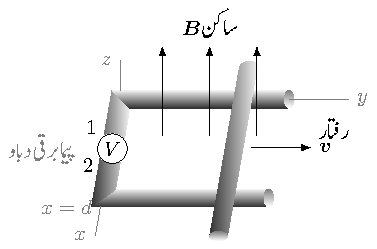
\includegraphics{figMaxwellSlidingConductorInStaticField}
\caption{وقت کے ساتھ نہ تبدیل ہوتے یکساں مقناطیسی میدان میں حرکت کرتے موصل سلاخ پر محرک برقی دباو پیدا ہوتی ہے۔}
\label{شکل_میکس_ویل_محرک_سلاخ_محرک_دباو}
\end{figure}

آئیں اب ایسی مثال دیکھیں جس میں وقت کے ساتھ تبدیل نہ ہونے والے مقناطیسی میدان میں  بند دائرہ حرکت کر رہا ہو۔شکل \حوالہ{شکل_میکس_ویل_محرک_سلاخ_محرک_دباو} میں ایسی صورت حال دکھائی گئی ہے۔اس شکل میں \عددیء{\kvec{v}} سمتی رفتار کو ظاہر کرتی ہے جبکہ \اصطلاح{پیما برقی دباو}\فرہنگ{پیما!برقی دباو}\فرہنگ{برقی دباو!پیما}\حاشیہب{voltmeter}\فرہنگ{voltmeter} کو \عددیء{V} سے  ظاہر کیا گیا ہے۔اس شکل میں دو افقی اور دو متوازی موصل سلاخ بند دائرہ یا بند دور بناتے ہیں۔ متوازی افقی سلاخوں کو بائیں طرف عمودی سلاخ سے جوڑا گیا ہے جس میں قابل نظر انداز جسامت اور لامحدود مزاحمت والا پیما برقی دباو نسب ہے، جبکہ دائیں جانب انہیں \عددیء{\kvec{v}} سمتی رفتار سے حرکت کرتے عمودی سلاخ سے جوڑا گیا ہے۔وقت کے ساتھ نہ تبدیل ہوتا اور ہر جگہ یکساں کثافت مقناطیسی بہاو \عددیء{\kvec{B}} بند دائرے کی گھیرے سطح کے عمودی ہے۔

مثبت \عددیء{\kvec{B}} کی صورت میں \عددیء{\kvec{B}} کی سمت ہی بند دائرے سے گھیری گئی سطح کی سمت ہو گی اور بند دائرے کی سمت گھڑی کے الٹ ہو گی۔یوں دائرے کے مثبت سمت میں دائیں ہاتھ کی انگلیاں رکھتے ہوئے گھیری سطح کی سمت انگوٹھے سے حاصل کی جاتی ہے۔ 

کسی بھی لمحہ \عددیء{t} پر حرکت کرتے سلاخ کے مقام کو \عددیء{y} سے ظاہر کرتے ہوئے ہم \عددیء{y=v t} لکھ سکتے ہیں جہاں \عددیء{v} سلاخ کے رفتار کی قیمت ہے۔یوں لمحہ \عددیء{t} پر بند دور کا ارتباط بہاو
\begin{align*}
\Phi=B d y =B d v t
\end{align*} 
ہو گا جو مساوات \حوالہ{مساوات_میکس_ویل_فیراڈے_قانون} کے تحت بند دور میں
\begin{align*}
e=-\frac{\dif \Phi}{\dif t}=-B d v
\end{align*}
محرک برقی دباو \عددیء{e} پیدا کرے گا۔

اب محرک برقی دباو \عددیء{\oint \kvec{E}\cdot \dif \kvec{L}} کو کہتے ہیں لہٰذا مندرجہ بالا جواب دائرے پر گھڑی کے الٹ سمت میں اس بند لکیری تکمل سے بھی حاصل ہونا چاہیے۔ہم دیکھ چکے ہیں کہ برقی سکون کی صورت میں موصل کی سطح پر سطح کے متوازی \عددیء{E} صفر رہتی ہے۔ہم آگے دیکھیں گے کہ وقت کے ساتھ تبدیل ہوتے برقی میدان میں بھی موصل کی سطح پر متوازی \عددیء{E} صفر ہی رہتی ہے۔یوں شکل \حوالہ{شکل_میکس_ویل_محرک_سلاخ_محرک_دباو} پر گھڑی کے الٹ چلتے ہوئے تمام سلاخوں پر تکمل کی قیمت صفر کے برابر ہو گی۔پیما برقی دباو کی مزاحمت صفر نہیں ہے لہٰذا تکمل کی قیمت پیما برقی دباو پر مندرجہ بالا قیمت کے برابر ہونا ہو گا۔گھڑی کی الٹ سمت چلتے ہوئے پیما برقی دباو کی لمبائی کو \عددیء{\dif \kvec{L}} لکھتے ہوئے ہم دیکھتے ہیں کہ \عددیء{\kvec{E} \cdot \dif \kvec{L}=-B d v} ہونا ہو گا۔چونکہ \عددیء{\dif \kvec{L}=\dif L \ax} کے برابر ہے لہٰذا \عددیء{\kvec{E}} کی سمت \عددیء{\ax} کے الٹ ہو گی۔یوں پیما برقی دباو پر \عددیء{\kvec{E}} کی سمت پیما کے دوسرے سرے سے پہلے سرے کی جانب ہے اور پیما پر برقی دباو کا مثبت سرا پیما کا دوسرا سرا ہے۔

پیما کی جگہ مزاحمت جوڑنے سے دور میں گھڑی کے الٹ برقی رو گزرے گی جو \عددیء{\az} کے الٹ سمت میں مقناطیسی بہاو پیدا کرے گی۔یہ لورنز کے قانون کے عین مطابق ہے۔

آئیں اب اسی شکل میں دئے مسئلے کو حرکی برقی دباو تصور کرتے ہوئے حل کریں۔مقناطیسی میدان میں \عددیء{\kvec{v}} سمتی رفتار سے حرکت کرتے ہوئے بار \عددیء{Q} پر قوت
\begin{align*}
\kvec{F}=Q \kvec{v} \times \kvec{B}
\end{align*}
یا حرکی شدت \عددیء{\kvec{E}_{\textrm{حرکی}}}
\begin{align}\label{مساوات_میکس_ویل_حرکی_برقی_شدت}
\kvec{E}_{\textrm{حرکی}}=\frac{\kvec{F}}{Q}=\kvec{v} \times \kvec{B}
\end{align}
عمل کرتی ہے۔حرکی شدت \عددیء{\ax} سمت میں ہے۔حرکت کرتے سلاخ میں ساکن مثبت ایٹم اور آزاد منفی الیکٹران پائے جاتے ہیں۔ان تمام باروں  پر ایسی قوت پائی جائے گی البتہ ساکن ایٹم مقید ہونے کی بنا حرکت نہیں کریں گے۔اگر محرک سلاخ کو متوازی سلاخوں سے اٹھایا جائے تو اس میں آزاد الیکٹران پر \عددیء{\ax} کے الٹ جانب قوت انہیں سلاخ کے پرلے سرے پر انبار کرنا شروع کر دے گی۔الیکٹرانوں کا انبار سلاخ میں \عددیء{-\ax} جانب برقی میدان کی شدت \عددیء{\kvec{E}_{\textrm{ساکن}}} پیدا کرے گا۔الیکٹران کا انبار بڑھتا رہے گا حتیٰ کہ  \عددیء{\kvec{E}_{\textrm{حرکی}}} اور \عددیء{\kvec{E}_{\textrm{ساکن}}} برابر ہو جائیں۔ایسا ہوتے ہی سلاخ میں کل برقی میدان کی شدت صفر ہو جائے گی اور اس میں بار کا حرکت رک جائے گا۔

یوں حرکی برقی دباو
\begin{align}\label{مساوات_میکس_ویل_حرکت_سے_دباو}
\textrm{\RL{محرک برقی دباو}}=\oint \kvec{E}_{\textrm{حرکی}} \cdot \dif \kvec{L}=\oint \left(\kvec{v} \times \kvec{B} \right) \cdot \dif \kvec{L}
\end{align} 
سے حاصل ہو گی۔مساوات کے دائیں ہاتھ بند دائرے کے ساکن حصوں پر تکمل کی قیمت صفر ہو گی لہٰذا محرک برقی دباو صرف حرکت کرتے حصوں کی وجہ سے پیدا ہو گی۔یوں حرکت کرتے سلاخ پر گھڑی کے الٹ چلتے ہوئے تکمل سے
\begin{align*}
\oint \left(\kvec{v} \times \kvec{B} \right) \cdot \dif \kvec{L}=\int_d^0 v B \dif x=-B v d
\end{align*}
حاصل ہوتا ہے ۔چونکہ \عددیء{\kvec{B}} از خود وقت کے ساتھ تبدیل نہیں ہو رہا لہٰذا یہی کل محرک برقی دباو ہو گا۔

یوں وقت کے ساتھ تبدیل نہ ہوتے مقناطیسی میدان میں حرکت کرتے بند دائرے میں محرک برقی دباو حاصل کرتے وقت حرکت کرتے حصوں پر حرکی شدت \عددیء{\kvec{E}_{\textrm{حرکی}}} کے استعمال سے محرک برقی دباو یوں
\begin{align}
\textrm{\RL{محرک برقی دباو}}=\oint \kvec{E} \cdot \dif \kvec{L}=\oint \kvec{E}_{\textrm{حرکی}} \cdot \dif \kvec{L}=\oint \left(\kvec{v} \times \kvec{B} \right) \cdot \dif \kvec{L}
\end{align} 
حاصل کی جا سکتی ہے۔البتہ وقت کے ساتھ بدلتی مقناطیسی میدان میں محرک برقی دباو کے حصول میں مساوات \حوالہ{مساوات_میکس_ویل_پہلی_مساوات_تکمل_صورت} کا حصہ شامل کرنا ضروری ہے یوں محرک برقی دباو
\begin{align}
\textrm{\RL{محرک برقی دباو}}=\oint \kvec{E} \cdot \dif \kvec{L}=-\int_S \frac{\partial \kvec{B}}{\partial t} \cdot \dif \kvec{S}+\oint \left(\kvec{v} \times \kvec{B} \right) \cdot \dif \kvec{L}
\end{align} 
سے حاصل ہو گی۔یہ مساوات دراصل مساوات \حوالہ{مساوات_میکس_ویل_فیراڈے_قانون}
\begin{align*}
\textrm{\RL{محرک برقی دباو}}=-\frac{\dif \Phi}{\dif t}
\end{align*}
ہی ہے۔

\begin{figure}
\centering
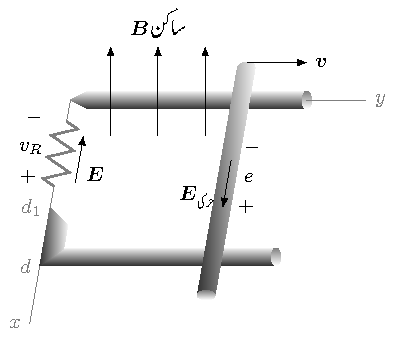
\includegraphics{figMaxwellDefiningElectromotiveForceEMF}
\caption{محرک برقی دباو اور برقی دباو کا موازنہ۔}
\label{شکل_میکس_ویل_محرک_دباو_اور_عام_دباو_موازنہ}
\end{figure}

آئیں شکل \حوالہ{شکل_میکس_ویل_محرک_سلاخ_محرک_دباو} میں پیما برقی دباو کی جگہ مزاحمت نسب کرتے ہوئے اس کی مدد سے  مساوات \حوالہ{مساوات_میکس_ویل_محرک_برقی_دباو_تعریف} جو محرک برقی دباو کی تعریف بیان کرتا ہے پر دوبارہ غور کریں۔نئی شکل کو شکل \حوالہ{شکل_میکس_ویل_محرک_دباو_اور_عام_دباو_موازنہ} میں دکھایا گیا ہے۔مساوات \حوالہ{مساوات_میکس_ویل_حرکی_برقی_شدت} محرک سلاخ پر پیدا \عددیء{\kvec{E}_{\textrm{حرکی}}} دیتا ہے جو سلاخ میں مثبت بار کو سلاخ کے اُرلے سرے کی طرف دھکیلے گا۔اس کے برعکس مزاحمت پر برقی دباو \عددیء{v_R} پایا جاتا ہے جس کی وجہ سے اس میں برقی میدان کی شدت \عددیء{\kvec{E}} پائی جائے گی جو مزاحمت میں مثبت بار کو مزاحمت کے پرلے سرے کی جانب دھکیلے گی۔

آپ شکل کو دیکھ کر تسلی کر لیں کہ مزاحمت پر میدان کی شدت \عددیء{\kvec{E}=-E\ax} سے برقی دباو \عددیء{v_R} یوں
\begin{align}
v_R=-\int_0^{d_1} \kvec{E} \cdot \dif \kvec{L}=\int_0^{d_1} E \dif x=E d_1
\end{align}
حاصل ہوتی ہے جبکہ متحرک سلاخ پر حرکی شدت \عددیء{\kvec{E}_{\textrm{حرکی}}=E_{\textrm{حرکی}}\ax} سے حرکی دباو \عددیء{e} یوں
\begin{align}
e=\oint \kvec{E}_{\textrm{حرکی}} \cdot \dif \kvec{L}=\int_0^d \kvec{E}_{\textrm{حرکی}} \cdot \dif \kvec{L}=\int_0^d E_{\textrm{حرکی}} \dif x=E_{\textrm{حرکی}}d
\end{align}
حاصل ہوتی ہے۔شکل میں دو افقی موصل سلاخوں کے مابین برقی دباو کو سلاخوں کے بائیں سروں پر \عددیء{v_R} جبکہ ان کے دائیں سروں پر \عددیء{e} کہا گیا ہے لہٰذا \عددیء{v_R} اور \عددیء{e} دونوں مثبت اور برابر قیمت رکھتے ہیں۔یہاں ضرورت اس بات کی ہے کہ آپ دیکھ سکیں کہ \عددیء{v_R} کی مثبت قیمت حاصل کرنے کے لئے ضروری ہے کہ مساوات میں منفی کی علامت استعمال کی جائے جبکہ \عددیء{e} کے مثبت قیمت کے حصول کے لئے ضروری ہے کہ مساوات میں جمع کی علامت استعمال کی جائے۔حرکی دباو کے بند تکمل میں دائرے کے بقایا اطراف پر تکمل کی قیمت صفر ہونے کے ناطے صرف متحرک سلاخ پر تکمل لیا گیا ہے۔


اگرچہ مساوات \حوالہ{مساوات_میکس_ویل_فیراڈے_قانون} انتہائی سادہ شکل رکھتی ہے لیکن اس کا استعمال کبھی کبھار مشکل ہو جاتا ہے۔ایسا اس وقت ہوتا ہے جب دور کے کسی حصے کو تبدیل کرتے ہوئے دوسرا حصہ نسب کیا جائے۔یہ بات شکل \حوالہ{شکل-میکس_ویل_سوئچ_سے_محرک_دباو_نہیں_پیدا_ہوتی} پر غور کرنے سے بہتر سمجھ آئے گی۔اس شکل میں نا تو وقت کے ساتھ تبدیل ہوتا مقناطیسی میدان ہے اور نا ہی بند دائرے کا کوئی حصہ متحرک ہے۔البتہ شکل میں دکھائے سوئچ کو چالو یا غیر چالو کرتے ہوئے بند دائرے میں مقناطیسی بہاو کم اور زیادہ کیا جا سکتا ہے۔یہاں بغیر سوچے مساوات \حوالہ{مساوات_میکس_ویل_فیراڈے_قانون} استعمال کرتے ہوئے غلط نتائج حاصل ہوتے ہیں۔ یاد رہے کہ برقی دباو یا تو وقت کے ساتھ بدلتے مقناطیسی میدان اور یا پھر بند دائرے کے کسی حصے کے حرکت سے ہی پیدا ہو گا۔
  
\begin{figure}
\centering
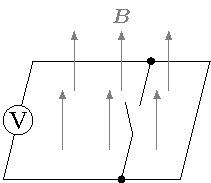
\includegraphics{figMaxwellSwitchingCoductorsToChangeFlux}
\caption{محرک برقی دباو یا تا وقت کے ساتھ بدلتی مقناطیسی میدان اور یا حرکت کرتے بند دائرے سے ہی پیدا ہو سکتی ہے۔}
\label{شکل-میکس_ویل_سوئچ_سے_محرک_دباو_نہیں_پیدا_ہوتی}
\end{figure}

%==============
\ابتدا{مشق}
خطہ \عددی{\rho<\SI{4}{\centi\meter}} میں میدان \عددی{\kvec{B}=\tfrac{2 \cos 1000 t \az}{5+\rho^2} \, \si{\tesla}} پایا جاتا ہے۔ الف) سطح \عددی{z=\SI{1.5}{\centi\meter}}، \عددی{\rho<\SI{2}{\centi\meter}} سے گزرتی مقناطیسی بہاو حاصل کریں۔ ب) نقطہ \عددی{N(0.02,10^{\circ},3)} پر \عددی{\kvec{E}} حاصل کریں۔ پ) سطح \عددی{z=0} پر رداس \عددی{\rho=\SI{2}{\centi\meter}} اور مزاحمت \عددی{\SI{4}{\ohm\per\centi\meter}} کی موصل تار کا دائرہ پایا جاتا ہے۔اس تار میں برقی رو حاصل کریں۔

جوابات: \عددی{502.6 \cos 1000t \, \si{\micro\weber}}، \عددی{4\sin 1000 t \aphi \, \si{\volt\per\meter}}، \عددی{10\sin 1000 t \, \si{\milli\ampere}}
\انتہا{مشق}
%==========================
\ابتدا{مشق}
شکل \حوالہ{شکل-میکس_ویل_سوئچ_سے_محرک_دباو_نہیں_پیدا_ہوتی} میں \عددیء{\kvec{B}=0.5\az } ٹسلا، رفتار \عددیء{100 y \ay} میٹر فی سیکنڈ جبکہ \عددیء{d=0.5} میٹر ہے۔اگر \عددیء{t=0} پر \عددیء{y=0.2} میٹر ہو تب \عددیء{t=15} ملی سیکنڈ پر مندرجہ ذیل حاصل کریں۔
\begin{itemize}
\item
سلاخ کی رفتار،
\item
محرک برقی دباو \عددیء{V_{21}}،
\item
پیما برقی دباو کی اندرونی مزاحمت دس میگا اوہم کی صورت میں دور میں برقی رو۔
\end{itemize} 

جوابات:\عددیء{\SI{4.017}{\meter\per\second}}، \عددیء{\SI{100}{\volt}}، \عددیء{\SI{10}{\micro \ampere}}

\انتہا{مشق}
%=======================

\حصہ{انتقالی برقی رو}
فیراڈے کے تجرباتی نتیجے سے میکس ویل کی پہلی مساوات
\begin{align}\label{مساوات_میکس_ویل_انتقالی_رو_الف}
\nabla \times \kvec{E}=-\frac{\partial \kvec{B}}{\partial t}
\end{align}
حاصل ہوئی جو کہتا ہے کہ بدلتی مقناطیسی میدان پیدا کرتا ہے برقی دباو۔گردش کے عمل کو مد نظر رکھتے ہوئے ہم دیکھتے ہیں ایسے پیدا کردہ برقی دباو کا بند لکیری تکمل صفر کے برابر نہیں ہوتا۔ آئیں اب وقت کے ساتھ تبدیل ہوتے برقی میدان پر غور کریں۔

ایمپیئر کے دوری قانون کی نقطہ شکل
\begin{align}\label{مساوات_میکس_ویل_ایمپیئر_دوری_نقطہ_صورت}
\nabla \times \kvec{H}=\kvec{J}
\end{align}
ساکن مقناطیسی میدان پر لاگو ہوتی ہے۔اس مساوات کی پھیلاو
\begin{align*}
\nabla \cdot \nabla \times \kvec{H}=0=\nabla \cdot \kvec{J}
\end{align*}
 لیتے ہوئے ہم دیکھتے ہیں کہ گردش کی پھیلاو ہر صورت صفر کے برابر ہوتی ہے لہٰذا مندرجہ بالا مساوات کا بایاں ہاتھ ہر صورت صفر دے گا اور یوں اگر یہ مساوات درست ہو تب اس کا دایاں ہاتھ بھی ہر صورت صفر ہونا چاہیے۔مگر ہم استمراری  مساوات سے جانتے ہیں کہ
\begin{align}
\nabla \cdot \kvec{J}=-\frac{\partial \rho}{\partial t}
\end{align} 
ہوتا ہے۔اس سے ثابت ہوتا ہے کہ مساوات \حوالہ{مساوات_میکس_ویل_ایمپیئر_دوری_نقطہ_صورت} صرف اس صورت درست ہو گا جب \عددیء{\tfrac{\partial \rho}{\partial t}=0} ہو۔یہ ایک غیر ضروری اور غیر حقیقی شرط ہے لہٰذا وقت کے ساتھ تبدیل ہوتے برقی میدان پر استعمال کے قابل بنانے کی خاطر  مساوات \حوالہ{مساوات_میکس_ویل_ایمپیئر_دوری_نقطہ_صورت} کو تبدیل کرنا لازم ہے۔تصور کریں کہ مساوات \حوالہ{مساوات_میکس_ویل_ایمپیئر_دوری_نقطہ_صورت} میں نا معلوم جزو \عددیء{\kvec{G}} کی شمولیت سے یہ مساوات وقت  کے ساتھ تبدیل ہوتے برقی میدان پر بھی لاگو کرنے کے قابل ہو جاتا ہے۔ایسی صورت میں مساوات \حوالہ{مساوات_میکس_ویل_ایمپیئر_دوری_نقطہ_صورت} یوں
\begin{align*}
\nabla \times \kvec{H}=\kvec{J}+\kvec{G}
\end{align*}
لکھی جائے گی۔آئیں دوبارہ اس کی پھیلاو حاصل کریں جس سے
\begin{align*}
0=\nabla \cdot \kvec{J}+\nabla \cdot \kvec{G}
\end{align*}
یا
\begin{align*}
\nabla \cdot \kvec{G}=\frac{\partial \rho}{\partial t}
\end{align*}
حاصل ہوتا ہے جہاں استمراری مساوات کا سہارا لیا گیا۔اس مساوات میں \عددیء{\rho} کی جگہ \عددیء{\nabla \cdot \kvec{D}} پر کرنے سے
\begin{align*}
\nabla \cdot \kvec{G}=\frac{\partial \left(\nabla \cdot \kvec{D} \right)}{\partial t}=\nabla \cdot \frac{\partial \kvec{D}}{\partial t}
\end{align*}
یعنی
 \begin{align*}
\kvec{G}=\frac{\partial \kvec{D}}{\partial t}
\end{align*}
حاصل ہوتا ہے۔یوں ایمپیئر کے دوری قانون کی درست شکل
\begin{align}\label{مساوات-میکس_ویل_دوسری_مساوات_نقطہ_شکل}
\nabla \times \kvec{H}=\kvec{J}+\frac{\partial \kvec{D}}{\partial t}
\end{align}
ہے۔ مندرجہ بالا مساوات برقی و مقناطیسیات کے اب تک تمام دریافت کردہ اصولوں پر پورا اترتی آئی ہے۔جب تک یہ غلط ثابت نہ ہو جائے، ہم اسے درست ہی تصور کریں گے۔

مساوات \حوالہ{مساوات-میکس_ویل_دوسری_مساوات_نقطہ_شکل} میکس ویل کے مساوات میں سے ایک مساوات ہے۔اس مساوات میں \عددیء{\tfrac{\partial \kvec{D}}{\partial t}} کی بُعد ایمپیئر فی مربع میٹر حاصل ہوتی ہے جو کثافت برقی رو کا بُعد ہے۔میکس ویل نے اس مساوات میں دائیں ہاتھ نئے جزو  کو \اصطلاح{کثافت انتقالی رو}\فرہنگ{کثافت!انتقالی رو}\فرہنگ{رو!کثافت انتقالی}\حاشیہب{displacement current density}\فرہنگ{displacement current density}\فرہنگ{current!displacement} کا نام دیا اور \عددیء{\kvec{J}_d} سے ظاہر کیا یعنی
\begin{gather}
\begin{aligned}\label{مساوات-میکس_ویل_دوسری_مساوات_نقطہ_شکل_ب}
\nabla \times \kvec{H}&=\kvec{J}+\kvec{J}_d\\
\kvec{J}_d&=\frac{\partial \kvec{D}}{\partial t}
\end{aligned}
\end{gather}

ہم تین اقسام کے کثافت رو دیکھ چکے جن میں کثافت انتقالی رو\فرہنگ{رو!انتقالی} کے علاوہ  غیر بار شدہ خطے میں عموماً الیکٹران کے حرکت سے پیدا  کثافت ایصالی رو\فرہنگ{رو!ایصالی}
\begin{align}
\kvec{J}=\sigma \kvec{E}
\end{align}
اور بار کے حجم کے حرکت سے پیدا کثافت اتصالی رو\فرہنگ{رو!اتصالی}
\begin{align}
\kvec{J}=\rho_h \kvec{v}
\end{align}
شامل ہیں۔مساوات \حوالہ{مساوات-میکس_ویل_دوسری_مساوات_نقطہ_شکل} میں \عددیء{\kvec{J}} سے مراد ایصالی اور اتصالی رو کے کثافتوں کا مجموعہ ہے جبکہ مقید بار \عددیء{\kvec{H}} کا حصہ ہیں۔غیر موصل خطے میں جہاں کثافت بار پائی ہی نہیں جاتی \عددیء{\kvec{J}=0} ہوتا ہے لہٰذا غیر موصل میں
\begin{align}\label{مساوات_میکس_ویل_مقناطیسی_شدت_گردش}
\nabla \times \kvec{H}=\frac{\partial \kvec{D}}{\partial t}  \quad \quad (\kvec{J}=0)
\end{align}
ہو گا۔مساوات \حوالہ{مساوات_میکس_ویل_مقناطیسی_شدت_گردش} اور مساوات \حوالہ{مساوات_میکس_ویل_انتقالی_رو_الف} میں مشابہت دیکھیں۔
\begin{align*}
\nabla \times \kvec{E}=-\frac{\partial \kvec{B}}{\partial t}
\end{align*} 
مقناطیسی شدت \عددیء{\kvec{H}} اور برقی شدت \عددیء{\kvec{E}} کافی مشابہت رکھتے ہیں۔ اسی طرح کثافت رو \عددیء{\kvec{D}} اور کثافت بہاو \عددیء{\kvec{B}} بھی کافی مشابہت رکھتے ہیں۔اس مشابہت کو یہیں تک رکھیں چونکہ جیسے ہی میدان میں بار پر قوت کی بات کی جائے، دونوں اقسام کے میدان بالکل مختلف طریقوں سے  عمل کرتے ہیں۔

کسی بھی سطح سے کل انتقالی رو سطحی تکمل
\begin{align}
I_d=\int_S \kvec{J}_d \cdot \dif \kvec{S}=\int_S \frac{\partial \kvec{D}}{\partial t} \cdot \dif \kvec{S}
\end{align}
سے حاصل ہو گی۔مساوات \حوالہ{مساوات-میکس_ویل_دوسری_مساوات_نقطہ_شکل} کے سطحی تکمل
\begin{align*}
\int_S \left(\nabla \times \kvec{H} \right) \cdot \dif \kvec{S}=\int_S \kvec{J} \cdot \dif \kvec{S}+\int_S \frac{\partial \kvec{D}}{\partial t} \cdot \dif \kvec{S}
\end{align*}
پر مسئلہ سٹوکس کے اطلاق سے
\begin{align}
\oint \kvec{H} \cdot \dif \kvec{L}=I+I_d=I+\int_S \frac{\partial \kvec{D}}{\partial t} \cdot \dif \kvec{S}
\end{align}
 وقت کے ساتھ تبدیل ہوتے ایمپیئر کے دوری قانون\فرہنگ{ایمپیئر قانون!عمومی نقطہ شکل} کی نقطہ شکل حاصل ہوتی ہے۔

\begin{figure}
\centering
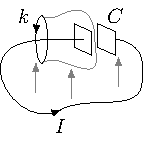
\includegraphics{figMaxwellConductionDisplacementCurrents}
\caption{موصل تار میں ایصالی رو برق گیر  کے چادروں کے درمیان انتقالی رو کے برابر ہے۔}
\label{شکل_میکس_ویل_ایصالی_انتقالی_رو}
\end{figure}

انتقالی رو کو شکل \حوالہ{شکل_میکس_ویل_ایصالی_انتقالی_رو} کی مدد سے سمجھتے ہیں جہاں موصل تار سے برق گیر  \عددیء{C} کے دو سرے جوڑتے ہوئے بند دور بنایا گیا ہے جس میں وقت کے ساتھ بدلتی سائن نما مقناطیسی میدان \عددیء{\kvec{B}} محرک برقی دباو
\begin{align*}
e=V_0 \cos \omega t
\end{align*}
 پیدا کرتی ہے۔یہ سادہ برقی دور ہے جس میں مزاحمت اور امالہ کو نظر انداز کرتے ہوئے برقی رو
\begin{align*}
i&=-\omega C V_0 \sin \omega t\\
&=-\omega \frac{\epsilon S}{d} V_0 \sin \omega t
\end{align*}
لکھی جا سکتی ہے جہاں \عددیء{\epsilon}، \عددیء{S} اور \عددیء{d} برق گیر (کپیسٹر) سے متعلق ہیں۔آئیں انتقالی رو کو نظرانداز کرتے ہوئے تار کے گرد بند دائرے  \عددیء{k} پر ایمپیئر کا دوری قانون لاگو کریں۔
\begin{align*}
\oint_k \kvec{H} \cdot \dif \kvec{L}=I_k
\end{align*}
اب بند دائرہ \عددیء{k} اور اس دائرے پر \عددیء{\kvec{H}} حقیقی مقدار ہیں اور تکمل سے حاصل رو \عددیء{I_k} اس دائرے سے گھیرے کسی بھی سطح سے گزرتی رو کو ظاہر کرتی ہے۔اگر ہم \عددیء{k} کو سیدھی سطح کا سرحد تصور کریں تب موصل تار اس سطح کو چھیدتا ہوا گزرے گا۔یوں اس سطح سے \عددیء{I} رو ہی گزرے گی جو ایصالی رو ہے۔اس کے برعکس اگر ہم \عددیء{k} کو تھیلے کا منہ تصور کریں جیسے شکل میں دکھایا گیا ہے تب ایصالی رو ایسی سطح سے نہیں گزرتی چونکہ تھیلا برق گیر (کپیسٹر)  کے دو چادروں کے درمیان سے گزرتا ہے اور تار اسے چھوتی تک نہیں۔ایسی صورت میں تھیلے سے گزرتی ایصالی رو صفر کے برابر ہے۔ایسی صورت میں ہمیں انتقالی رو کا سہارا لینا ہو گا۔برق گیر (کپیسٹر)  کے چادروں کے درمیان
\begin{align*}
D=\epsilon E=\epsilon \left(\frac{V_0}{d} \cos \omega t \right)
\end{align*}
ہے لہٰذا
\begin{align*}
J_d=\frac{\partial D}{\partial t}=-\omega \epsilon \frac{V_0}{d} \sin \omega t
\end{align*}
اور یوں
\begin{align*}
I_d=S J_d =-\omega \frac{\epsilon  S}{d} V_0\sin \omega t 
\end{align*}
ہو گی۔

یہ وہی جواب ہے جو ایصالی رو سے حاصل ہوا تھا۔اس مثال سے آپ دیکھ سکتے ہیں کہ ایمپیئر کے دوری قانون کو استعمال کرتے ہوئے سطح سے  گزرتی ایصالی رو اور انتقالی رو دونوں کا خیال رکھنا ہو گا۔کہیں پر سطح سے صرف ایصالی رو گزرے گی تو کہیں اس سے صرف انتقالی رو گزرے گی اور کبھی کبھار دونوں کا مجموعہ۔

انتقالی رو وقت کے ساتھ بدلتے برقی میدان سے پیدا ہوتے ہیں لہٰذا یہ ایسے تمام غیر موصل یا نیم موصل خطوں میں پائی جاتی ہے جہاں وقت کے ساتھ تبدیل ہوتی ایصالی رو پائی جائے۔اگرچہ موصل خطے میں بھی انتقالی رو پائی جاتی ہے لیکن، جیسے آپ مندرجہ ذیل مشق میں دیکھیں گے، اس کی قیمت ایصالی رو کی نسبت سے اتنی کم ہوتی ہے کہ یہ قابل نظر انداز ہوتی ہے۔یہی وجہ ہے کہ انتقالی رو تجرباتی طور دریافت نہیں کی گئی بلکہ اس تک منطق کے ذریعہ سے پہنچا گیا۔

%=====================
\ابتدا{مثال}
ایک خطے کے مستقل \عددی{\sigma=0}، \عددی{\mu_R=2.5} اور \عددی{\epsilon_R=1.2} ہیں۔اس میں کثافت انتقالی برقی رو درج ذیل ہے۔
\begin{align*}
\kvec{J}_d=10\cos(2\times 10^8 t - k x) \ay \, \si{\micro\ampere\per\meter\squared}
\end{align*}
الف) \عددی{\kvec{D}} اور \عددی{\kvec{E}} حاصل کریں۔ ب) فیراڈے کے قانون کی نقطہ شکل اور تکمل کے استعمال کرتے ہوئے \عددی{\kvec{B}} اور \عددی{\kvec{H}} حاصل کریں۔ پ) مساوات \حوالہ{مساوات-میکس_ویل_دوسری_مساوات_نقطہ_شکل_ب} استعمال کرتے ہوئے \عددی{\kvec{J}_d} حاصل کریں۔ ت) حاصل \عددی{\kvec{J}_d} اور سوال میں دیے  گئے \عددی{\kvec{J}_d} کا آپس میں موازنہ کرتے ہوئے \عددی{k} کی مثبت قیمت حاصل کریں۔

حل:الف)  چونکہ \عددی{\kvec{J}_d=\tfrac{\partial \kvec{D}}{\partial t}} کے برابر ہے لہٰذا
\begin{align*}
\kvec{D}=\int \kvec{J}_d \dif t=5\times 10^{-14} \sin (2\times 10^8 t - k x) \ay +M \quad \si{\coulomb \per\meter\squared}
\end{align*}
حاصل کیا جا سکتا ہے۔ساکن میدان صفر ہونے کی صورت میں تکمل کا مستقل \عددی{M=0} ہو گا۔یوں
\begin{align*}
\kvec{E}=\frac{\kvec{D}}{\epsilon_R \epsilon_0}=4.7\times 10^{-3} \sin (2\times 10^8 t - k x) \ay \quad \si{\volt\per\meter}
\end{align*}
ہو گا۔

ب) فیراڈے کے قانون سے
\begin{align*}
\nabla \times \kvec{E}=-4.70587111\times 10^{-3} k \cos (2\times 10^8 t - k x) \az=-\frac{\partial \kvec{B}}{\partial t}
\end{align*}
لکھتے ہوئے تکمل لے کر
\begin{align*}
\kvec{B}=\int 4.70587111\times 10^{-3} k \cos (2\times 10^8 t - k x) \az \dif t=2.3529\times 10^{-11} k \sin(2\times 10^8 t - k x) \az
\end{align*}
حاصل ہوتا ہے جس سے
\begin{align*}
\kvec{H}=\frac{\kvec{B}}{\mu_R \mu_0}=7.4896\times 10^{-6} k \sin(2\times 10^8 t - k x) \az
\end{align*}
لکھا جا سکتا ہے۔

پ) چونکہ \عددی{\sigma=0} ہے لہٰذا کثافت ایصالی برقی رو صفر ہو گی۔یوں مساوات \حوالہ{مساوات-میکس_ویل_دوسری_مساوات_نقطہ_شکل_ب} سے \عددی{} حاصل کرتے ہیں۔
\begin{align*}
\nabla \times \kvec{H}=7.4896 \times 10^{-6} k^2 \cos (2\times 10^8 t - k x) \ay \, \si{\ampere\per\meter\squared}=\kvec{J}_d
\end{align*}

ت) حاصل کردہ اور سوال میں دیا گیا \عددی{\kvec{J}_d} برابر پر کرتے ہوئے
\begin{align*}
k=\sqrt{\frac{10\times 10^{-6}}{7.4896\times 10^{-6}}}=\SI{1.155}{\meter^{-1}}
\end{align*}
حاصل ہوتا ہے۔

\انتہا{مثال}
%=====================
\ابتدا{مثال}
رداس \عددی{a} اور \عددی{b} کے موصل ہم محوری کرہ، جہاں \عددی{b>a} ہے، کو برقی دباو \عددی{v=V_0\cos \omega t} مہیا کی جاتی ہے۔دونوں کرہ کے درمیانی خطے کے مستقل \عددی{\sigma=0}، \عددی{\epsilon_R=1} اور \عددی{\mu_R=1} ہیں۔بیرونی کرہ کو برقی زمین تصور کریں۔ الف)  کرہ برق گیر (کپیسٹر)  کو مہیا برقی رو حاصل کریں۔ ب) دونوں کرہ کے مابین انتقالی برقی رو حاصل کریں۔ پ) کیا بیرون برق گیر (کپیسٹر)  ایصالی برقی رو اور اندرون برق گیر (کپیسٹر)  انتقالی برقی رو برابر ہیں؟

حل: الف) صفحہ \حوالہصفحہ{مساوات_کپیسٹر_ہم_محوری_کرہ} پر مساوات \حوالہ{مساوات_کپیسٹر_ہم_محوری_کرہ} کرہ کپیسٹر کی کپیسٹنس دیتی ہے جس سے مہیا کردہ ایصالی برقی رو یوں
\begin{align*}
I=C\frac{\dif v}{\dif t}=-\frac{4\pi\epsilon \omega V_0}{\frac{1}{a}-\frac{1}{b}} \sin \omega t
\end{align*}
حاصل کی جا سکتی ہے۔

ب) صفحہ \حوالہصفحہ{مساوات_لاپلاس_کروی_رداسی_لاپلاسی_دباو} پر مساوات \حوالہ{مساوات_لاپلاس_کروی_رداسی_لاپلاسی_دباو} استعمال کرتے ہوئے دونوں کرہ کے درمیان خطے میں برقی دباو کو
\begin{align*}
V=\frac{\frac{1}{r}-\frac{1}{b}}{\frac{1}{a}-\frac{1}{b}} V_0 \cos \omega t
\end{align*}
لکھتے ہوئے 
\begin{align*}
\kvec{E}&=-\nabla V=\frac{V_0 \cos \omega t}{r^2\left(\frac{1}{a}-\frac{1}{b}\right)}  \, \ar\\
\kvec{D}&=\epsilon \kvec{E}=\frac{\epsilon V_0 \cos \omega t}{r^2\left(\frac{1}{a}-\frac{1}{b}\right)} \, \ar
\end{align*}
حاصل ہوتا ہے جس سے کثافت انتقالی برقی رو  
\begin{align*}
\kvec{J}=\frac{\partial \kvec{D}}{\partial t}=-\frac{\omega \epsilon V_0 \sin \omega t}{r^2\left(\frac{1}{a}-\frac{1}{b}\right)} \, \ar
\end{align*}
لکھی جا سکتی ہے۔یوں انتقالی برقی رو
\begin{align*}
I_d=4\pi r^2 J_d=-\frac{4 \pi \omega \epsilon V_0 \sin \omega t}{\left(\frac{1}{a}-\frac{1}{b}\right)} 
\end{align*}
ہو گی۔

پ) بیرون برق گیر (کپیسٹر)  ایصالی برقی رو اور اندرون برق گیر (کپیسٹر)  انتقالی برقی رو برابر ہیں۔
\انتہا{مثال}
%===================
\ابتدا{مشق}
ٹھوس تانبے کی تار میں سائن نما، پچاس ہرٹز کی ایصالی رو \عددیء{I_0 \cos \omega t} گزر رہی ہے۔اس میں انتقالی رو حاصل کریں۔پچاس ہرٹز رو کی صورت میں ایصالی اور انتقالی رو کے موثر قیمت کی شرح حاصل کریں۔

حل:\عددیء{I_d=-\tfrac{\omega \epsilon_0}{\sigma} I_0\sin \omega t} جبکہ ان کے موثر قیمت کی شرح  \عددیء{\tfrac{I}{I_d}=\tfrac{\sigma}{\omega \epsilon_0}=\num{2.08e16}} ہے۔

\انتہا{مشق}
%====================

\حصہ{میکس ویل مساوات کی نقطہ شکل}\شناخت{حصہ_میکس_ویل_میکس_ویل_نقطہ_اشکال}
ہم وقت کے ساتھ تبدیل ہوتے میدانوں میں میکس ویل کے دو مساوات کے نقطہ اشکال\فرہنگ{میکس ویل!نقطہ اشکال}\فرہنگ{Maxwell's equation!point form}
\begin{align}\label{مساوات-میکس_ویل_تفرقی_الف}
\nabla \times \kvec{E}=-\frac{\partial \kvec{B}}{\partial t}
\end{align}
اور
\begin{align}\label{مساوات-میکس_ویل_تفرقی_ب}
\nabla \times \kvec{H}=\kvec{J}+\frac{\partial \kvec{D}}{\partial t}
\end{align}
 حاصل کر چکے ہیں۔میکس ویل کے بقایا دو مساوات وقت کے ساتھ تبدیل ہوتے میدان میں بھی جوں کے توں
\begin{align}
\nabla \cdot \kvec{D}&=\rho_h \label{مساوات_میکس_ویل_گاوس_قانون_نقطہ}\\
\nabla \cdot \kvec{B}&=0 \label{مساوات_میکس_ویل_مقناطیسی_میدان_دو_قطب}
\end{align}
 رہتے ہیں۔ 

مساوات \حوالہ{مساوات_میکس_ویل_گاوس_قانون_نقطہ} کہتا ہے کہ کثافت برقی رو کا منبع کثافت بار  ہے۔وقت کے ساتھ بدلتے مقناطیسی میدان میں برقی میدان  پیدا ہوتا ہے جو بند دائرے پر چلتا ہے۔ایسے برقی میدان کا نا تو کسی بار سے اخراج ہوتا ہے اور نا ہی یہ کسی بار پر ختم ہوتا ہے۔اس کے برعکس ہر مثبت بار سے اس کے برابر برقی بہاو کا اخراج ہوتا ہے اور ہر منفی بار پر اس کے برابر برقی بہاو کا اختتام ہوتا ہے۔
  

مساوات \حوالہ{مساوات_میکس_ویل_مقناطیسی_میدان_دو_قطب} کہتا ہے کہ کسی بھی نقطے سے کل مقناطیسی بہاو کا اخراج صفر ہے یعنی مقناطیسی بہاو نا تو کسی نقطے سے خارج ہوتا ہے اور نا ہی یہ کسی نقطے پر اختتام پذیر ہوتا ہے۔ سادہ زبان میں اس کا مطلب ہے کہ مقناطیس کا یک قطب ممکن نہیں جس سے مقناطیسی بہاو کا اخراج ہو یا اس پر مقناطیسی بہاو اختتام ہو۔

مندرجہ بالا چار مساوات پر برقی و مقناطیسیات کی بنیاد کھڑی ہے جنہیں استعمال کرنے کی خاطر چار معاون مساوات
\begin{align}
\kvec{D}&=\epsilon \kvec{E} \label{مساوات_میکس_ویل_خالی_خلاء_برقی_مستقل}\\
\kvec{B}&=\mu \kvec{H} \label{مساوات_میکس_ویل_خالی_خلاء_مقناطیسی_مستقل}\\
\kvec{J}&=\sigma \kvec{E}\\
\kvec{J}&=\rho_h \kvec{v}
\end{align}
بھی درکار ہوتے ہیں۔

ایسے ذو برق اور مقناطیسی اشیاء جن میں متغیرات سادہ تعلق نہ رکھتے ہوں، ان میں مساوات \حوالہ{مساوات_میکس_ویل_خالی_خلاء_برقی_مستقل} اور مساوات \حوالہ{مساوات_میکس_ویل_خالی_خلاء_مقناطیسی_مستقل} کی جگہ
\begin{align}
\kvec{D}&=\epsilon_0 \kvec{E}+\kvec{P}\\
\kvec{B}&=\mu_0 \left(\kvec{H}+\kvec{M} \right)
\end{align}
استعمال ہوتے ہیں۔خطی اشیاء میں
\begin{align}
\kvec{P}=\chi_e \kvec{E}
\end{align}
اور
\begin{align}
\kvec{M}=\chi_m \kvec{H}
\end{align}
لکھا جا سکتا ہے۔

آخر میں لورنز قوت کی مساوات 
\begin{align}
\kvec{F}=\rho_h \left(\kvec{E}+\kvec{v} \times \kvec{B} \right)
\end{align}
بھی شامل کرتے ہیں۔

غیر سمتی مقناطیسی دباو \عددیء{V} اور سمتی مقناطیسی دباو \عددیء{\kvec{A}} انتہائی اہم ہیں البتہ ان کی شمولیت لازم نہیں۔
%===================
\ابتدا{مثال}
ایک خطے میں \عددی{\rho_h=0} ہے۔اگر اس خطے میں \عددی{\nabla \cdot \kvec{E}=0} ہو تب خطے کی برقی مستقل \عددی{\epsilon} پر کیا شرط لاگو ہوتی ہے۔

حل: مساوات \حوالہ{مساوات_میکس_ویل_گاوس_قانون_نقطہ} کے تحت \عددی{\rho_h=0} کی صورت میں \عددی{\nabla \cdot \kvec{D}=0} ہو گا۔یوں
\begin{align*}
\nabla \cdot \kvec{D}=\nabla \cdot (\epsilon \kvec{E})==\kvec{E} \cdot \nabla \epsilon+\epsilon \nabla \cdot \kvec{E}=0
\end{align*}
یا
\begin{align*}
\nabla \cdot \kvec{E}+\kvec{E} \cdot \frac{\nabla \epsilon}{\epsilon}=0
\end{align*}
لکھا جا سکتا ہے۔اب \عددی{\nabla \cdot \kvec{E}=0} اس صورت ہو گا اگر \عددی{\nabla \epsilon=0} ہو۔
\انتہا{مثال}
%=====================
\ابتدا{مشق}
ایک خطے کے مستقل \عددی{\sigma=0}، \عددی{\epsilon_R=2.5} اور \عددی{\mu_R=10} ہیں۔کیا اس خطے میں میدان \عددی{\kvec{D}=(z+6\times 10^7 t)\ax} اور \عددی{\kvec{B}=(-754z-4.52\times 10^{10}t)\ay} کی جوڑی میکس ویل کے مساوات پر پورا اترتے ہیں۔

جواب:چونکہ برقی میدان سے حاصل \عددی{\nabla \times \kvec{E}} مقناطیسی میدان سے حاصل \عددی{-\tfrac{\partial \kvec{B}}{\partial t}} کے برابر ہے اور اسی طرح مقناطیسی میدان سے حاصل  \عددی{\nabla \times \kvec{H}} مقناطیسی میدان سے حاصل \عددی{\tfrac{\partial \kvec{D}}{\partial t}} کے برابر ہے لہٰذا یہ جوڑی میکس ویل کے مساوات پر پورا اترتی ہے۔
\انتہا{مشق}
%===================
\حصہ{میکس ویل مساوات کی تکمل شکل}
 مساوات \حوالہ{مساوات-میکس_ویل_تفرقی_الف} کے سطحی تکمل پر مسئلہ سٹوکس کے اطلاق سے فیراڈے کے  قانون کو
\begin{align}\label{مساوات_میکس_ویل_تکمل_مساوات_الف}
\oint \kvec{E} \cdot \dif \kvec{L}=-\int_S \frac{\partial \kvec{B}}{\partial t} \cdot \dif \kvec{S}
\end{align}
لکھا جا سکتا ہے۔اسی طرح مساوات \حوالہ{مساوات-میکس_ویل_تفرقی_ب} سے ایمپیئر کے دوری قانون کی تکمل صورت
\begin{align}\label{مساوات_میکس_ویل_تکمل_مساوات_ب}
\oint \kvec{H} \cdot \dif \kvec{L}=I+\int_S \frac{\partial \kvec{D}}{\partial t} \cdot \dif \kvec{S}
\end{align}
حاصل ہوتی ہے۔

برقی اور مقناطیسی میدان کے تکمل اشکال، گاوس کے قوانین مساوات \حوالہ{مساوات_میکس_ویل_گاوس_قانون_نقطہ} اور مساوات \حوالہ{مساوات_میکس_ویل_مقناطیسی_میدان_دو_قطب} کے حجمی تکمل اور مسئلہ پھیلاو کی مدد سے یوں لکھے جا سکتے ہیں۔ 
\begin{align}\label{مساوات_میکس_ویل_تکمل_مساوات_پ}
\oint_S \kvec{D} \cdot \dif \kvec{S}=\int_h \rho_h \dif h
\end{align}
اور
\begin{align}\label{مساوات_میکس_ویل_تکمل_مساوات_ت}
\oint_S \kvec{B} \cdot \dif \kvec{S}=0
\end{align}

مندرجہ بالا چار مساوات سے \عددیء{\kvec{E}}، \عددیء{\kvec{H}}، \عددیء{\kvec{D}} اور \عددیء{\kvec{B}} کے سرحدی شرائط حاصل ہوتے ہیں جن سے میکس ویل کے جزوی تفرقی مساوات کے مستقل حاصل کئے جاتے ہیں۔وقت کے ساتھ تبدیل ہوتے میدان کے سرحدی شرائط عموماً ساکن میدان کے سرحدی شرائط ہی ہوتے ہیں لہٰذا ساکن میدان کے طریقہ کار سے وقت کے ساتھ بدلتے میدان کے سرحدی شرائط بھی حاصل کئے جا سکتے ہیں۔

\begin{figure}
\centering
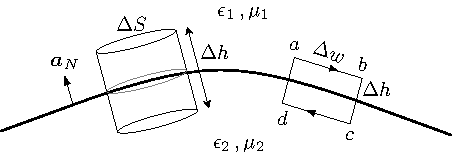
\includegraphics{figMaxwellBoundaryConditions}
\caption{وقت کے ساتھ بدلتے میدان کے سرحدی شرائط۔}
\label{شکل_میکس_ویل_سرحدی_شرائط}
\end{figure}

آئیں شکل \حوالہ{شکل_میکس_ویل_سرحدی_شرائط}  کی مدد سے  سرحد کے متوازی برقی اور مقناطیسی شرائط\فرہنگ{سرحدی شرائط!برقی اور مقناطیسی}\فرہنگ{برقی میدان!سرحدی شرائط}\فرہنگ{مقناطیسی میدان!سرحدی شرائط}\فرہنگ{boundary conditions! electric and magnetic}\فرہنگ{electric field!boundary conditions}\فرہنگ{magnetic field!boundary conditions} حاصل کریں۔ شکل میں مستطیل دائرے پر مساوات \حوالہ{مساوات_میکس_ویل_تکمل_مساوات_الف} کے اطلاق سے
\begin{align*}
\left(E_{m1}-E_{m2}\right) \Delta w=-\frac{\partial B_{n}}{\partial t}  \Delta w \Delta h
\end{align*}  
لکھا جا سکتا ہے جہاں \عددیء{\tfrac{\partial B_{n}}{\partial t}} سے مراد دائرے کے گھیرے سطح سے گزرتی مجموعی میدان کی تبدیلی ہے جس کا کچھ حصہ خطہ \عددیء{1} اور کچھ حصہ خطہ \عددیء{2} سے گزرتا ہے۔اس مساوات کے دائیں ہاتھ کی قیمت \عددیء{\Delta h \to 0} کرتے ہوئے صفر کے قریب تر کی جا سکتی ہے۔ایسی صورت میں دائیں ہاتھ کو صفر ہی تصور کرتے ہوئے
\begin{align}\label{مساوات_میکس_ویل_سرحدی_شرائط_بدلتے_میدان_الف}
E_{m1}=E_{m2}
\end{align}
یعنی
\begin{align}
\aN \times \left(\kvec{E}_1-\kvec{E}_2 \right)=0
\end{align}
حاصل ہوتا ہے۔

سرحد پر انتہائی کم موٹائی کے خطے میں کثافت برقی رو \عددیء{\kvec{K}} تصور کرتے ہوئے کسی بھی چھوٹی لمبائی \عددیء{\dif \kvec{L}} پر برقی رو کو \عددیء{I=\kvec{K} \cdot \dif \kvec{L}} لکھا جا سکتا ہے۔یوں شکل \حوالہ{شکل_میکس_ویل_سرحدی_شرائط} میں مستطیل دائرے پر مساوات \حوالہ{مساوات_میکس_ویل_تکمل_مساوات_ب} کے اطلاق سے
\begin{align*}
\left(H_{m1}-H_{m2} \right) \Delta w=K_\perp \Delta w +\frac{\partial D}{\partial t} \Delta w \Delta h
\end{align*}
حاصل ہوتا ہے جہاں \عددیء{K_\perp} سے مراد \عددیء{K} کا وہ حصہ ہے جو \عددیء{H_{m1}} اور \عددیء{H_{m2}} کے عمودی ہے۔دائیں ہاتھ دوسرے جزو کی قیمت \عددیء{\Delta h \to 0} کرتے ہوئے صفر کے قریب تر کی جا سکتی ہے لہٰذا اس جزو کو نظرانداز کرتے ہوئے
\begin{align}\label{مساوات_میکس_ویل_متوازی_مقناطیسی_موج_سرحدی_شرط}
H_{m1}-H_{m2}=K_\perp
\end{align}
حاصل ہوتا ہے جسے یوں
\begin{align}
\aN \times \left(\kvec{H}_1-\kvec{H}_2 \right)=\kvec{K}_\perp
\end{align}
بھی لکھا جا سکتا ہے۔

کسی بھی حقیقی دو مختلف اشیاء کے سرحد، مثلاً سمندر کے پانی اور ہوا کے سرحد یا ہوا اور دیوار کے سرحد، پر کثافت برقی رو \عددیء{\kvec{K}} صفر ہوتی ہے۔لہٰذا حقیقی مسائل میں \عددیء{K=0} کی بنا پر
\begin{align}\label{مساوات_میکس_ویل_سرحدی_شرائط_بدلتے_میدان_ب}
H_{m1}=H_{m2}
\end{align}
ہو گا۔صفحہ \حوالہصفحہ{شکل_امالہ_مقناطیسی_سرحدی_شرائط} پر شکل \حوالہ{شکل_امالہ_مقناطیسی_سرحدی_شرائط} میں سطحی کثافت برقی رو \عددیء{\kvec{K}} دکھائی گئی ہے جبکہ یہاں شکل \حوالہ{شکل_میکس_ویل_سرحدی_شرائط} میں اسے صفر تصور کرتے ہوئے نہیں دکھایا گیا۔

مساوات \حوالہ{مساوات_میکس_ویل_تکمل_مساوات_پ} اور مساوات \حوالہ{مساوات_میکس_ویل_تکمل_مساوات_ت} سے سرحدی عمودی شرائط
\begin{align}\label{مساوات_میکس_ویل_سرحدی_شرائط_بدلتے_میدان_پ}
\aN \cdot \left(\kvec{D}_1-\kvec{D}_2 \right)&=\rho_S
\end{align}
اور
\begin{align}\label{مساوات_میکس_ویل_سرحدی_شرائط_بدلتے_میدان_ت}
\aN \cdot \left(\kvec{B}_1-\kvec{B}_2 \right)=0
\end{align}
حاصل ہوتے ہیں۔

موصل کو ایسا کامل موصل تصور کرتے ہوئے جس کی موصلیت لامحدود مگر \عددیء{\kvec{J}} محدود ہو سے موصل کے اندر اوہم کے قانون سے
\begin{align}
\kvec{E}=0
\end{align}
اور یوں فیراڈے کے قانون کی نقطہ شکل سے، وقت کے ساتھ تبدیل ہوتے میدان کی صورت میں
\begin{align}
\kvec{H}=0
\end{align}
حاصل ہوتے ہیں۔اس طرح ایمپیئر کے دوری قانون کی نقطہ شکل سے محدود \عددیء{\kvec{J}} کی قیمت
\begin{align}
\kvec{J}=0
\end{align}
حاصل ہوتی ہے لہٰذا برقی رو صرف موصل کی سطح پر بطور سطحی کثافت رو \عددیء{\kvec{K}} ممکن ہے۔یوں اگر خطہ \عددیء{2} کامل موصل ہو تب مساوات \حوالہ{مساوات_میکس_ویل_سرحدی_شرائط_بدلتے_میدان_الف}، \حوالہ{مساوات_میکس_ویل_سرحدی_شرائط_بدلتے_میدان_ب}، \حوالہ{مساوات_میکس_ویل_سرحدی_شرائط_بدلتے_میدان_پ} اور \حوالہ{مساوات_میکس_ویل_سرحدی_شرائط_بدلتے_میدان_ت} کی جگہ
\begin{align}
E_{m1}&=0   \label{مساوات_میکس_ویل_کامل_موصل_سرحدی_شرط_الف}\\
H_{m1}&=K   \label{مساوات_میکس_ویل_کامل_موصل_سرحدی_شرط_ب}\\
D_{n1}&=\rho_S    \label{مساوات_میکس_ویل_کامل_موصل_سرحدی_شرط_پ}\\
B_{n1}&=0    \label{مساوات_میکس_ویل_کامل_موصل_سرحدی_شرط_ت}
\end{align}
لکھا جائے گا۔یاد رہے کہ سطحی کثافت بار کی موجودگی ذو برق، کامل موصل اور غیر کامل موصل تمام پر ممکن ہے جبکہ سطحی کثافت رو \عددیء{\kvec{K}} صرف کامل موصل کی صورت میں ممکن ہے۔

مندرجہ بالا سرحدی شرائط میکس ویل کے مساوات کے حل کے لئے لازم  ہیں۔حقیقت میں پیش آنے والے تمام مسائل میں مختلف اشیاء کے سرحدیں پائی جاتی ہیں اور ایسے ہر سرحد کے دونوں اطراف پر مختلف متغیرات کے تعلق سرحدی شرائط سے ہی حاصل کرنا ممکن ہے۔کامل موصل کی صورت میں موصل کے اندر،  وقت کے ساتھ بدلتے، تمام متغیرات صفر ہوتے ہیں البتہ ایسی صورت میں مساوات \حوالہ{مساوات_میکس_ویل_کامل_موصل_سرحدی_شرط_الف} تا مساوات \حوالہ{مساوات_میکس_ویل_کامل_موصل_سرحدی_شرط_ت} میں دئے شرائط کا اطلاق نہایت مشکل ہوتا ہے۔

لامحدود خطے کو بے سرحد خطہ تصور کیا جا سکتا ہے۔سرحد کی غیر موجودگی میں متحرک لہروں کے چند بنیادی خاصیت لہر کی حرکت پر غور سے واضح ہوتے ہیں۔اگلا باب انہیں متحرک لہروں پر ہے۔چونکہ لامحدود خطے میں سرحد نہیں پایا جاتا لہٰذا سرحدی شرائط کی ضرورت نہیں پڑتی۔اسی وجہ سے لامحدود خطے میں میکس ویل مساوات کا حل نہایت آسان ہوتا ہے۔ 
%=====================
\ابتدا{مثال}
موصل سطح پر نقطہ \عددی{N(2,3-1)} پایا جاتا ہے جہاں میدان \عددی{\kvec{E}=(15\ax-20\ay+6\az)\cos 10^6 t \, \si{\volt\per\meter}} ہے۔موصل سطح کے گرد خطے کے مستقل \عددی{\mu_R=2.2}، \عددی{\epsilon_R=1.6} اور \عددی{\sigma=0} ہیں۔ الف) نقطہ \عددی{N} پر موصل سطح کی عمودی اکائی سمتیہ \عددی{\aN} حاصل کریں۔ ب) اس نقطے پر کثافت بار حاصل کریں۔

حل:الف) چونکہ نقطہ \عددی{N} پر برقی میدان دیا گیا ہے اور موصل سطح پر برقی میدان سطح کے عمودی ہوتا ہے لہٰذا عمودی سمتیہ \عددی{\kvec{E}} کے سمت میں ہی ہو گا۔یوں لمحہ \عددی{t=0} پر میدان کی قیمت استعمال کرتے ہوئے \عددی{\aN} حاصل کرتے ہیں۔
\begin{align*}
\aN=\frac{\kvec{E}_{t=0}}{\abs{\kvec{E}_{t=0}}}&=\frac{15\ax-20\ay+6\az }{\sqrt{15^2+20^2+6^2}}=0.58\ax-0.78\ay+0.23\az
\end{align*}

ب) موصل سطح پر عمودی میدان اور کثافت بار کے تعلق سے
\begin{align*}
\rho_S=\kvec{D} \cdot \aN&=1.6\epsilon_0 (15\ax-20\ay+6\az)\cos 10^6 t \cdot (0.58\ax-0.78\ay+0.23\az)\\
&=1.138 \cos(10^6 t) \, \si{\nano \coulomb \per\meter\squared}
\end{align*}
حاصل ہوتا ہے۔
\انتہا{مثال}
%=======================
\ابتدا{مثال}
خطہ-1 کے مستقل \عددی{\sigma_1=0}، \عددی{\epsilon_{R1}=5.2} اور \عددی{\mu_{R1}=6} ہیں جبکہ خطہ-2 کے مستقل \عددی{\sigma_2=0}، \عددی{\epsilon_{R2}=1.5} اور \عددی{\mu_{R2}=2.2} ہیں۔ان کے سرحد پر کوئی کثافت بار نہیں پایا جاتا۔ سمتیہ \عددی{10\ax-5\ay+15\az} خطہ-2 سے خطہ-1 کی جانب ہے۔خطہ الف میں سرحد کے قریب نقطہ \عددی{N} پر میدان \عددی{\kvec{E}_1=(100\ax-50\ay+80\az) \cos 3600 t \, \si{\volt\per\meter}} پایا جاتا ہے۔ الف) اسی نقطے کے قریب \عددی{ٰE_{t1}}، \عددی{E_{n2}} اور \عددی{E_2} حاصل کریں۔

جوابات:\عددی{\SI{41.8}{\volt\per\meter}}، \عددی{\SI{454}{\volt\per\meter}}، \عددی{\SI{456}{\volt\per\meter}}
\انتہا{مثال}
%======================
\ابتدا{مثال}
\عددی{z<0} خطہ-1 ہے جہاں \عددی{\epsilon_1=\SI{1.5e-11}{\farad\per\meter}}، \عددی{\mu_1=\SI{2.2e-6}{\henry\per\meter}} اور \عددی{\sigma_1=\SI{6e-3}{\siemens\per\meter}} ہیں۔خطہ-2 جو \عددی{z>0} پر پایا جاتا ہے میں \عددی{\epsilon_2=2\epsilon_1}، 
\عددی{\mu_2=\tfrac{\mu_1}{2}} اور \عددی{\sigma_2=4\sigma_1} ہیں۔نقطہ \عددی{N(0,0,0^-)} سرحد پر خطہ-1 میں پایا جاتا ہے جہاں میدان
 \عددی{\kvec{E}_1=(30\ax+20\ay+10\az)\cos 10^9 t \, \si{\volt\per\meter}} ہے۔الف)اس نقطے پر \عددی{\kvec{E}_{n1}}، \عددی{\kvec{E}_{m1}}، \عددی{\kvec{D}_{n1}} اور \عددی{\kvec{D}_{m1}} حاصل کریں۔ ب) اس نقطے پر \عددی{\kvec{J}_{n1}} اور \عددی{\kvec{J}_{m1}} حاصل کریں۔ پ) اسی نقطے پر \عددی{\kvec{E}_{m2}}، \عددی{\kvec{D}_{m2}} اور \عددی{\kvec{J}_{m2}} حاصل کریں۔ ت) استمراری مساوات کی مدد
 سے \عددی{J_{n1}-J_{n2}=-\tfrac{\partial D_{n1}}{\partial t}+\tfrac{\partial D_{n2}}{\partial t}} لکھتے ہوئے \عددی{D_{n2}}، \عددی{J_{n2}} اور \عددی{E_{n2}} حاصل کریں۔

حل:الف) خطہ-1 سے خطہ-2 جانب اکائی سمتیہ \عددی{\az} ہے۔ یوں
\begin{align*}
E_{n1}&=\aN \cdot \kvec{E}_1=\az \cdot [30 \ax+20\ay+10\az] \cos (10^9 t) =10 \cos (10^9 t)
\end{align*}
ہو گا جس سے
\begin{align*}
\kvec{E}_{n1}&=E_{n1} \aN=10 \cos (10^9 t) \az\\
\kvec{E}_{m1}&=\kvec{E}_1-\kvec{E}_{n1}=[30\ax+20\ay]\cos (10^9 t)\\
\kvec{D}_{n1}&=\epsilon_1 \kvec{E}_{n1}=1.5\times 10^{-10}\cos (10^9 t) \az\\
\kvec{D}_{m1}&=\epsilon_1 \kvec{E}_{m1}=10^{-10} [4.5\ax+3\ay]\cos(10^9 t)
\end{align*}
لکھے جا سکتے ہیں۔

ب) 
\begin{align*}
\kvec{J}_{n1}&=\sigma_1 \kvec{E}_{n1}=(6\times 10^{-3})10 \cos (10^9 t) \az=\frac{3}{50}\cos (10^9 t)\az\\
\kvec{J}_{m1}&=\sigma_1 \kvec{E}_{m1}=(6\times 10^{-3})[30\ax+20\ay]\cos (10^9 t)=\left[\frac{9}{50}\ax+\frac{3}{25}\ay\right]\cos (10^9 t)
\end{align*}

پ) سرحد پر متوازی برقی میدان بے جوڑ ہوتا ہے لہٰذا اس سرحدی شرط کی بنا پر
\begin{align*}
\kvec{E}_{m2}=\kvec{E}_{m1}=[30\ax+20\ay]\cos (10^9 t)
\end{align*}
ہو گا جس سے 
\begin{align*}
\kvec{D}_{m2}&=\epsilon_2 \kvec{E}_{m2}=(3\times 10^{-11})[30\ax+20\ay]\cos (10^9 t)=10^{-10}[9\ax+6\ay]\cos (10^9 t)\\
\kvec{J}_{m2}&=\sigma_2 \kvec{E}_{m2}=(24\times 10^{-3})[30\ax+20\ay]\cos (10^9 t)=\left[\frac{18}{25}\ax+\frac{12}{25}\ay\right]\cos (10^9 t)
\end{align*}
حاصل کئے جا سکتے ہیں۔

ت) مساوات \حوالہ{مساوات_میکس_ویل_سرحدی_شرائط_بدلتے_میدان_پ} سرحد پر سطحی کثافت بار \عددی{\rho_S} اور عمودی میدان کا تعلق بیان کرتی ہے۔شکل \حوالہ{شکل_میکس_ویل_سرحدی_شرائط} کی طرح سرحد پر کم سے کم قد \عددی{(\Delta h \to 0)} کی چھوٹی ڈبیا میں کل \عددی{\rho_S \Delta S} بار پایا جائے گا۔اس ڈبیا سے برقی رو کی اخراج سے ڈبیا میں موجود بار میں کمی پیدا ہو گی جسے استمراری مساوات پیش کرتی ہے
\begin{align*}
(\kvec{J}_{n1}-\kvec{J}_{n2}) \cdot \Delta \kvec{S} = -\frac{\partial \rho_S}{\partial t} \Delta S
\end{align*}
جہاں \عددی{\rho_S=J_{n1}-J_{n2}} کے برابر ہے۔اس  مساوات کو 
\begin{align*}
J_{n1}-J_{n2}&=-\frac{\partial}{\partial t} (D_{n1}-D_{n2})
\end{align*}
یا
\begin{align*}
\sigma_1 E_{n1}-\sigma_2 E_{n2}=-\frac{\partial }{\partial t} (\epsilon_1 E_{n1}-\epsilon_2 E_{n2})
\end{align*}
لکھا جا سکتا ہے۔اس تفرقی مساوات میں \عددی{E_{n1}=10\cos 10^9 t} پر کرتے ہوئے \عددی{E_{n2}} کے لئے حل کرتے ہیں۔ایسا نا معلوم مستقل کے طریقے سے کرتے ہیں۔یہ طریقہ استعمال کرتے ہوئے ہم تصور کرتے ہیں کہ
\begin{align*}
E_{n2}=A \cos 10^9 t + B \sin 10^9 t
\end{align*}
کے برابر ہے جہاں \عددی{A} اور \عددی{B} درکار مستقل ہیں۔ ہم \عددی{E_{n1}} اور \عددی{E_{n2}} کو استمراری مساوات میں پر کرتے ہیں۔
\begin{multline*}
(6\times 10^{-3}) 10 \cos 10^9 t -24\times 10^{-3} [A \cos 10^9 t +B \sin 10^9 t]\\
=1.5\times 10^{-11} \times 10 \times 10^9 \sin 10^9 t+3\times 10^{-11}[-10^9 A \sin 10^9 t +10^9 B \cos 10^9 t ]
\end{multline*}
اس مساوات میں دونوں جانب \عددی{\cos} اجزاء کے سر برابر ہوں گے۔یوں
\begin{align*}
(6\times 10^{-3}) 10 -24 \times 10^{-3}A = 3\times 10^{-11} [10^9 B]
\end{align*}
ہو گا۔اسی طرح مساوات کے دونوں جانب \عددی{\sin} اجزاء کے سر برابر ہوں گے لہٰذا
\begin{align*}
-24\times 10^{-3}[B]=1.5\times 10^{-11} \times 10 \times 10^9+3\times 10^{-11}[-10^9 A]
\end{align*}
ہو گا۔مندرجہ بالا دو مساوات کو آپس میں حل کرتے ہوئے
\begin{align*}
A&=\frac{165}{41}\\
B&=-\frac{50}{41}
\end{align*}
حاصل ہوتا ہے جس سے 
\begin{align*}
E_{n2}=\frac{165}{41}\cos 10^9 t -\frac{50}{41}\sin 10^9 t=4.21 \cos (10^9 t -16.9^{\circ})
\end{align*}
لکھا جا سکتا ہے۔یوں
\begin{align*}
\kvec{E}_{n2}&=4.21 \cos (10^9 t -16.9^{\circ})\az\\
\kvec{D}_{n2}&=\epsilon_2 \kvec{E}_{n2}=(3\times 10^{-11})4.21 \cos (10^9 t -16.9^{\circ})\az=1.26\times 10^{-10}\cos (10^9t -16.9^{\circ})\az \\
\kvec{J}_{n2}&=\sigma_2 \kvec{E}_{n2}=(24\times 10^{-3})4.21 \cos (10^9 t -16.9^{\circ})\az=0.1\cos (10^9 t -16.9^{\circ})\az
\end{align*}
ہوں گے۔
\انتہا{مثال}
%=====================
\حصہ{تاخیری دباو}
وقت کے ساتھ بدلتے دباو، جنہیں \اصطلاح{تاخیری دباو}\فرہنگ{تاخیری دباو}\حاشیہب{retarded potentials}\فرہنگ{retarded potentials} کہا جاتا ہے، \اصطلاح{اشعاعی اخراج}\فرہنگ{اشعاعی اخراج}\حاشیہب{radiation}\فرہنگ{radiation}  کے مسائل حل کرنے میں نہایت اہم ثابت ہوتے ہیں۔آپ کو یاد ہو گا کہ غیر سمتی مقناطیسی دباو \عددیء{V} کو خطے میں تقسیم ساکن بار کی صورت
\begin{align}\label{مساوات_میکس_ویل_بدلتا_میدان_غیر_سمتی_دباو}
V=\int_h \frac{\rho_h \dif  h}{4 \pi \epsilon R} \quad \quad (\textrm{\RL{برقی سکون}})
\end{align}
میں لکھا جا سکتا ہے۔اسی طرح سمتی مقناطیسی دباو \عددیء{\kvec{A}} کو وقت کے ساتھ نہ بدلتے یعنی یک سمتی برقی رو کے تقسیم کی صورت
\begin{align}\label{مساوات_میکس_ویل_بدلتا_میدان_سمتی_دباو}
\kvec{A}=\int_h \frac{\mu \kvec{J} \dif h}{4\pi R} \quad \quad (\textrm{\RL{یک سمتی رو}})
\end{align}
میں لکھا جا سکتا ہے۔انہیں مساوات کے نقطہ اشکال بالترتیب
\begin{align}\label{مساوات_میکس-ویل_بدلتا_میدان_مساوات_الف}
\nabla^2 V=-\frac{\rho_h}{\epsilon}  \quad \quad (\textrm{\RL{برقی سکون}})
\end{align}
اور
\begin{align}\label{مساوات_میکس-ویل_بدلتا_میدان_مساوات_ب}
\nabla^2 \kvec{A}=-\mu \kvec{J}   \quad \quad (\textrm{\RL{یک سمتی رو}})
\end{align}
ہیں۔

غیر سمتی اور سمتی مقناطیسی دباو کے حصول کے بعد میدان کے بنیادی متغیرات ڈھلوان
\begin{align}\label{مساوات_میکس-ویل_بدلتا_میدان_مساوات_پ}
\kvec{E}=-\nabla V  \quad \quad (\textrm{\RL{برقی سکون}})
\end{align}
اور گردش
\begin{align}\label{مساوات_میکس-ویل_بدلتا_میدان_مساوات_ت}
\kvec{B}=\nabla \times \kvec{A}   \quad \quad (\textrm{\RL{یک سمتی رو}})
\end{align}
کی مدد سے حاصل ہوتے ہیں۔

آئیں اب ساکن بار اور یک سمتی رو سے متعلق، وقت کے ساتھ تبدیل ہوتے ایسے دباو حاصل کریں جو مندرجہ بالا مساوات پر پورا اترتے ہوں۔

میکس ویل کے مساوات کے تحت \عددیء{\nabla \cdot \kvec{B}=0} ہو گا۔صفحہ \حوالہصفحہ{مساوات_مقناطیسی_گردش_کی_پھیلاو_صفر_ہے} پر مساوات \حوالہ{مساوات_مقناطیسی_گردش_کی_پھیلاو_صفر_ہے} کے تحت گردش کی پھیلاو لازماً صفر ہوتی ہے لہٰذا مساوات \حوالہ{مساوات_میکس-ویل_بدلتا_میدان_مساوات_ت} میکس ویل کی مساوات \عددیء{\nabla \cdot \kvec{B}=0} پر پورا اترتی ہے۔ یوں ہم مساوات \حوالہ{مساوات_میکس-ویل_بدلتا_میدان_مساوات_ت} کو بدلتے میدان کے لئے بھی درست تصور کرتے ہیں۔


صفحہ \حوالہصفحہ{مشق_مقناطیسی_ڈھلوان_کی_گردش-صفر} پر مشق \حوالہ{مشق_مقناطیسی_ڈھلوان_کی_گردش-صفر} میں آپ نے ثابت کیا کہ ڈھلوان کی گردش لازماً صفر ہوتی ہے یوں مساوات \حوالہ{مساوات_میکس-ویل_بدلتا_میدان_مساوات_پ} کی گردش لینے سے دایاں ہاتھ صفر حاصل ہوتا ہے جبکہ بایاں ہاتھ \عددیء{\nabla \times \kvec{E}} حاصل ہوتا ہے جو مساوات \حوالہ{مساوات-میکس_ویل_تفرقی_الف} کے تحت صفر نہیں ہے۔یوں صاف ظاہر ہے کہ مساوات \حوالہ{مساوات_میکس-ویل_بدلتا_میدان_مساوات_پ} وقت کے ساتھ بدلتے میدان کے لئے درست نہیں ہے۔آئیں اس توقع سے مساوات \حوالہ{مساوات_میکس-ویل_بدلتا_میدان_مساوات_پ} کے دائیں جانب متغیرہ \عددیء{\kvec{N}} جمع کریں
\begin{align*}
\kvec{E}=-\nabla V +\kvec{N}
\end{align*}
 کہ وقت کے ساتھ بدلتے میدان کے لئے ایسی مساوات درست ثابت ہو گی۔ فی الحال \عددیء{\kvec{N}} ایک نا معلوم متغیرہ ہے۔گردش لینے سے
\begin{align*}
\nabla \times \kvec{E}=-\frac{\partial \kvec{B}}{\partial t} &=-\nabla \times \left( \nabla V\right) +\nabla \times \kvec{N}\\
&=0+\nabla \times \kvec{N}
\end{align*}
یعنی

\begin{align*}
\nabla \times \kvec{N}=-\frac{\partial \kvec{B}}{\partial t}
\end{align*}
حاصل ہوتا ہے۔مساوات \حوالہ{مساوات_میکس-ویل_بدلتا_میدان_مساوات_ت} کے استعمال سے یوں
\begin{align*}
\nabla \times \kvec{N}=-\frac{\partial }{\partial t} \left(\nabla \times \kvec{A} \right)
\end{align*}
یا
\begin{align*}
\nabla \times \kvec{N}=-\nabla \times \left(\frac{\partial \kvec{A}}{\partial t} \right)
\end{align*}
حاصل ہوتا ہے جس کا سادہ ترین حل
\begin{align*}
\kvec{N}=-\frac{\partial \kvec{A}}{\partial t}
\end{align*}
ہے لہٰذا اب ہم
\begin{align}\label{مساوات_میکس-ویل_بدلتا_میدان_مساوات_ٹ}
\kvec{E}=-\nabla V -\frac{\partial \kvec{A}}{\partial t}
\end{align}
 لکھ سکتے ہیں۔

ہمیں اب بھی دیکھنا ہو گا کہ آیا مساوات \حوالہ{مساوات_میکس-ویل_بدلتا_میدان_مساوات_ت} اور مساوات \حوالہ{مساوات_میکس-ویل_بدلتا_میدان_مساوات_ٹ} میکس ویل  کے بقایا دو مساوات یعنی مساوات \حوالہ{مساوات-میکس_ویل_تفرقی_ب} 
\begin{align*}
\nabla \times \kvec{H}&=\kvec{J}+\frac{\partial \kvec{D}}{\partial t}
\end{align*}
اور مساوات \حوالہ{مساوات_میکس_ویل_گاوس_قانون_نقطہ}
\begin{align*}
\nabla \cdot \kvec{D}=\rho_h
\end{align*}
پر پورا اترتے ہیں کہ نہیں۔یہاں پہلی مساوات میں \عددیء{\kvec{H}=\tfrac{1}{\mu}\nabla \times \kvec{A}} اور  \عددیء{\kvec{D}=\epsilon \kvec{E}} پر کرتے ہوئے 
\begin{align*}
\nabla \times \nabla \times \kvec{A}&=\kvec{J}+\epsilon \frac{\partial \kvec{E}}{\partial t}\\
&=\kvec{J}+\epsilon\left(-\nabla \frac{\partial V}{\partial t}- \frac{\partial^2 \kvec{A}}{\partial t^2} \right) 
\end{align*}
یا
\begin{align}\label{مساوات_میکس_ویل_بدلتی_ج}
\nabla \left(\nabla \cdot \kvec{A} \right)-\nabla^2 \kvec{A}=\mu \kvec{J}-\mu \epsilon \left(\nabla \frac{\partial V}{\partial t}+ \frac{\partial^2 \kvec{A}}{\partial t^2} \right)
\end{align}
لکھا جا سکتا ہے جہاں مساوات \حوالہ{مساوات_میکس-ویل_بدلتا_میدان_مساوات_ٹ} کا سہارا لیا گیا۔اسی طرح مساوات \حوالہ{مساوات_میکس_ویل_گاوس_قانون_نقطہ} سے
\begin{align*}
\epsilon \left(-\nabla \cdot \nabla V -\frac{\partial}{\partial t}\nabla \cdot  \kvec{A} \right)=\rho_h
\end{align*}
یا
\begin{align}\label{مساوات_میکس_ویل_بدلتی_چ}
\nabla^2 V+\frac{\partial}{\partial t} \left(\nabla \cdot \kvec{A} \right)=-\frac{\rho_h}{\epsilon}
\end{align}

حاصل ہوتا ہے۔

مساوات \حوالہ{مساوات_میکس_ویل_بدلتی_ج} اور مساوات \حوالہ{مساوات_میکس_ویل_بدلتی_چ} میں کوئی تضاد  نہیں پایا جاتا۔ساکن یا یک سمتی حالات میں \عددیء{\nabla \cdot \kvec{A}=0} کی وجہ سے  مساوات \حوالہ{مساوات_میکس_ویل_بدلتی_ج} اور مساوات \حوالہ{مساوات_میکس_ویل_بدلتی_چ} سے بالترتیب مساوات \حوالہ{مساوات_میکس-ویل_بدلتا_میدان_مساوات_ب} اور مساوات \حوالہ{مساوات_میکس-ویل_بدلتا_میدان_مساوات_الف} حاصل ہوتے ہیں۔یوں ہم فرض کر سکتے ہیں کہ وقت کے ساتھ بدلتے دباو کی تعریف یوں کی جا سکتی ہے کہ ان سے \عددیء{\kvec{B}} اور \عددیء{\kvec{E}} بذریعہ مساوات \حوالہ{مساوات_میکس-ویل_بدلتا_میدان_مساوات_ت} اور مساوات \حوالہ{مساوات_میکس-ویل_بدلتا_میدان_مساوات_ٹ} حاصل کئے جا سکتے ہوں۔البتہ \عددیء{\kvec{A}} اور \عددیء{V} کو مساوات \حوالہ{مساوات_میکس-ویل_بدلتا_میدان_مساوات_ت} اور مساوات \حوالہ{مساوات_میکس-ویل_بدلتا_میدان_مساوات_ٹ} از خود مکمل طور پر بیان نہیں کرتے۔یہ دو مساوات لازمی لیکن نا مکمل شرائط ہیں جن پر \عددیء{\kvec{A}} اور \عددیء{V} کا پورا اترنا ضروری ہے۔آئیں ایک مثال سے اس حقیقت کو سمجھیں۔

تصور کریں کہ ہمارے پاس سادہ سمتی مقناطیسی دباو ہے جس کے \عددیء{A_y} اور \عددیء{A_z} اجزاء صفر کے برابر ہیں۔ یوں مساوات \حوالہ{مساوات_میکس-ویل_بدلتا_میدان_مساوات_ت} کی مدد سے ہم لکھ سکتے ہیں۔
\begin{align*}
B_x \ax+B_y \ay+B_z \az=0\ax+\frac{\partial A_x}{\partial z}\ay-\frac{\partial A_x}{\partial y}\az
\end{align*}
اس سے ظاہر ہے کہ \عددیء{x} محدد کے ساتھ \عددیء{A_x} کے تبدیلی کے بارے میں کچھ اخذ کرنا ممکن نہیں ہے۔یہ مساوات \عددیء{\tfrac{\partial A_x}{\partial x}} کا ذکر تک نہیں کرتا۔ہاں اگر ہمیں \عددیء{\kvec{A}} کے پھیلاو کے بارے میں بھی معلومات فراہم ہوتی تب \عددیء{x} محدد کے ساتھ \عددیء{A_x} کے تبدیلی کے بارے میں کچھ کہنا ممکن ہوتا چونکہ دئے گئے سمتی دباو سے
\begin{align*}
\nabla \cdot \kvec{A}=\frac{\partial A_x}{\partial x}
\end{align*} 
لکھا جا سکتا ہے۔آخر میں یہ بھی بتانا ضروری ہے کہ \عددیء{\kvec{A}} کے بارے میں ہماری تمام معلومات جزوی تفرقی مساوات کی صورت میں ہیں  جن سے \عددیء{\kvec{A}} کے حصول کے وقت تکمل کا مستقل شامل کرنا ضروری ہے۔کسی بھی حقیقی مسئلہ جس میں مکمل خلاء کے لئے حل درکار ہو میں ایسا مستقل صفر کے برابر ہو گا چونکہ کوئی بھی میدان لا محدود فاصلے  پر صفر ہی ہو گا۔

اس مثال سے ہم کہہ سکتے ہیں کہ اگر ہمیں لامحدود خلاء میں کسی بھی نقطے پر سمتی میدان کی قیمت معلوم ہو تب اس سمتی میدان کو تمام خلاء میں میدان  کے گردش اور پھیلاو سے حاصل کیا جا سکتا ہے۔ہمیں مکمل آزادی ہے کہ جیسے چاہیں \عددیء{\kvec{A}} کی پھیلاو بیان کریں۔ ہم مساوات \حوالہ{مساوات_میکس_ویل_بدلتی_ج} اور مساوات \حوالہ{مساوات_میکس_ویل_بدلتی_چ} کو مدنظر رکھتے ہوئے یوں \عددیء{\kvec{A}} کے پھیلاو کے لئے سادہ ترین تفاعل
\begin{align}
\nabla \cdot \kvec{A}=-\mu \epsilon \frac{\partial V}{\partial t}
\end{align}
 لکھتے ہیں جس سے مساوات \حوالہ{مساوات_میکس_ویل_بدلتی_ج}
\begin{align}
\nabla^2 \kvec{A}=-\mu \kvec{J}+\mu \epsilon \frac{\partial^2 \kvec{A}}{\partial t^2}
\end{align}
صورت اختیار کر لے گی جبکہ مساوات \حوالہ{مساوات_میکس_ویل_بدلتی_چ}
\begin{align}
\nabla^2 V=-\frac{\rho_h}{\epsilon}+\mu \epsilon \frac{\partial^2 V}{\partial t^2}
\end{align}
صورت اختیار  کر لے گی۔

مندرجہ بالا دو مساوات متحرک امواج سے متعلق ہیں جن پر اگلے باب میں غور کیا جائے گا۔ان مساوات کی مشابہت بھی حیرت انگیز ہے۔باب کے اس حصے میں، وقت کے ساتھ بدلتے میدان کے لئے، حاصل کئے گئے نتائج یہاں دوبارہ پیش کرتے ہیں۔
\begin{align}
\kvec{B}=\nabla \times \kvec{A}   \label{مساوات_میکس_ویل_تاخیری_مقناطیسی_میدان}\\
\nabla \cdot \kvec{A}=-\mu \epsilon \frac{\partial V}{\partial t}\\
\kvec{E}=-\nabla V-\frac{\partial \kvec{A}}{\partial t}  \label{مساوات_میکس_ویل_تاخیری_برقی_میدان}
\end{align} 

اگلے باب میں متحرک امواج پر غور کیا جائے گا۔آپ دیکھیں گے کہ وقت کے ساتھ بدلتے برقی و مقناطیسی میدان متحرک امواج پیدا کرتے ہیں جن کی رفتار \عددیء{v}
\begin{align}
v=\frac{1}{\sqrt{\mu \epsilon}}
\end{align} 
کے برابر ہوتی ہے۔خالی خلاء میں یہ رفتار تقریباً \عددیء{\SI{3e8}{\meter \per \second}} کے برابر ہوتی ہے جو خالی خلاء میں روشنی کی رفتار ہے۔اس سے اخذ کیا جا سکتا ہے کہ نقطہ \عددیء{N_1} پر کثافت بار سے دور کسی نقطے \عددیء{N_2} پر دباو کی قیمت اسی لمحے کثافت بار کے قیمت پر منحصر نہیں ہوتی بلکہ کچھ دیر قبل کے کثافت بار پر منحصر ہوتی ہے۔کثافت بار میں تبدیلی کی خبر \عددیء{N_1} سے \عددیء{N_2} تک رفتار \عددیء{v} سے پہنچتی ہے لہٰذا ان نقطوں کے درمیان فاصلہ \عددیء{R} ہونے کی صورت میں یہ خبر \عددیء{\tfrac{R}{v}} سیکنڈ تاخیر سے پہنچے گی۔اس طرح وقت کے ساتھ بدلتی صورت میں مساوات  \حوالہ{مساوات_میکس_ویل_بدلتا_میدان_غیر_سمتی_دباو} کی نئی شکل
\begin{align}\label{مساوات_میکس_ویل_تاخیری_غیر_سمتی_دباو}
V=\int_h \frac{[\rho_h]}{4\pi \epsilon R} \dif h
\end{align}
ہو گی جہاں \عددیء{[\rho_h]} سے مراد یہ ہے کہ مساوات میں وقت \عددیء{t} کی جگہ تاخیری وقت \عددیء{t'} استعمال کیا جائے یعنی
\begin{align*}
t'=t-\frac{R}{v}
\end{align*}

یوں اگر خلاء میں کثافت بار
\begin{align*}
\rho_h=e^{-r} \cos \omega t
\end{align*}
ہو تب
\begin{align*}
[\rho_h]=e^{-r} \cos \left[\omega \left(t-\frac{R}{v} \right) \right]
\end{align*}
ہو گا جہاں \عددیء{R} تفرقی بار سے اس نقطے تک فاصلہ ہے جہاں اس تفرقی بار سے پیدا دباو کا حصول درکار ہو۔

اسی طرح وقت کے ساتھ بدلتی صورت میں مساوات \حوالہ{مساوات_میکس_ویل_بدلتا_میدان_سمتی_دباو} کی نئی شکل یعنی تاخیری سمتی مقناطیسی دباو کی مساوات
\begin{align}\label{مساوات_میکس_ویل_تاخیری_سمتی_دباو}
\kvec{A}=\int_h \frac{\mu [\kvec{J}]}{4\pi R} \dif h
\end{align}
ہو گی۔

تاخیری وقت کے استعمال کی بنا پر ایسے دباو کو \اصطلاح{تاخیری دباو}\فرہنگ{تاخیری دباو}\فرہنگ{دباو!تاخیری}\حاشیہب{retarded potential}\فرہنگ{retarded potential} کہا جاتا ہے۔

تاخیری برقی اور تاخیری مقناطیسی دباو کے استعمال سے برقی و مقناطیسی مسئلے نسبتاً زیادہ آسانی سے حل ہوتے ہیں۔یوں اگر ہمیں \عددیء{\rho} اور \عددیء{\kvec{J}} معلوم ہوں تب ہم مساوات \حوالہ{مساوات_میکس_ویل_تاخیری_غیر_سمتی_دباو} اور مساوات \حوالہ{مساوات_میکس_ویل_تاخیری_سمتی_دباو} سے \عددیء{V} اور \عددیء{\kvec{A}} حاصل کر سکتے ہیں جن سے مقناطیسی میدان بذریعہ مساوات \حوالہ{مساوات_میکس_ویل_تاخیری_مقناطیسی_میدان} اور برقی میدان بذریعہ مساوات \حوالہ{مساوات_میکس_ویل_تاخیری_برقی_میدان} حاصل کئے جا سکتے ہیں۔اگر ہمیں \عددیء{\rho} اور \عددیء{\kvec{J}} کی قیمتیں معلوم نہ ہوں اور نا ہی ان کے قیمتوں کا اندازہ لگانا ممکن ہو تب تاخیری دباو، میکس ویل مساوات کے حل سے زیادہ، مددگار ثابت نہیں ہوتے۔ 

\newpage
\حصہء{سوالات}

\ابتدا{سوال}
رداس \عددی{\rho=\SI{12}{\centi\meter}} کے گول دائرے میں وقت کے ساتھ تبدیل ہوتا، یکساں مقناطیسی میدان \عددی{B(t)=0.15\sin 1000 t \, \si{\weber}} ہے جو دائرے میں محرک برقی دباو \عددی{e(t)} پیدا کرتا ہے۔گول دائرے کی مزاحمت \عددی{\SI{55}{\ohm}} ہے۔محرک برقی دباو،  گول دائرے میں برقی رو \عددی{i(t)} پیدا کرتی ہے۔برقی رو \عددی{i(t)} سے پیدا مقناطیسی بہاو کو نظر انداز کرتے ہوئے \عددی{e(t)} اور \عددی{i(t)} حاصل کریں۔صورت حال شکل \حوالہ{شکل_سوال_میکس_ویل_دائرہ_محرک_دباو} میں دکھائی گئی ہے جہاں صفحہ سے اوپر کی جانب باہر نکلتی مقناطیسی میدان کو چھوٹے دائروں میں بند نقطوں سے ظاہر کیا گیا ہے۔
\begin{figure}
\centering
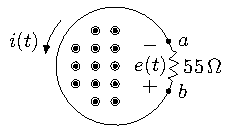
\includegraphics{figMaxwellRingEMF}
\caption{دائرے میں یکساں مقناطیسی بہاو، محرک برقی دباو پیدا کرتا ہے۔}
\label{شکل_سوال_میکس_ویل_دائرہ_محرک_دباو}
\end{figure}

جوابات:\عددی{-6.78 \cos 1000t \, \si{\volt}}، \عددی{-123\cos 1000t \, \si{\milli\ampere}}
\انتہا{سوال}
%======================
\ابتدا{سوال}
سطح \عددی{z=0} پر موصل تار کے مستطیل کے اطراف \عددی{x=\mp \SI{2}{\meter}}، \عددی{y=\mp\SI{1.5}{\meter}} پر ہیں۔وقت کے ساتھ تبدیل ہوتا مقناطیسی میدان \عددی{\kvec{B}=(0.25\ax-0.55\ay+0.1\az)\sin 1200 t \, \si{\tesla}} ہے۔مستطیل کی کل مزاحمت \عددی{R=\SI{4200}{\ohm}} ہے۔مثبت \عددی{z} محدد کی جانب سے دیکھتے ہوئے، گھڑی کی سمت میں برقی رو حاصل کریں۔برقی رو سے پیدا ثانوی مقناطیسی میدان کو نظر انداز کرتے ہوئے حل کریں۔

جواب:\عددی{343 \cos 1200 t \, \si{\milli\ampere}} 
\انتہا{سوال}
%=======================
\ابتدا{سوال}
مقناطیسی میدان \عددی{\kvec{B}=5\cos(1.2\times 10^{8} \pi t -\pi y)\az \, \si{\micro \tesla}} ہے۔مندرجہ ذیل فرضی یا غیر موصل دائروں پر \عددی{\aphi} سمت میں بڑھتا محرک برقی دباو حاصل کریں۔الف) \عددی{(0,0,0)} تا \عددی{(1,0,0)} تا \عددی{(1,1,0)} تا \عددی{(0,1,0)} تا \عددی{(0,0,0)}؛ ب) \عددی{(0,0,0)} تا \عددی{(2,0,0)} تا \عددی{(2,2,0)} تا \عددی{(0,2,0)} تا \عددی{(0,0,0)} 

جوابات:\عددی{600[\cos(1.2\times 10^{8} \pi t -\pi)-\cos (1.2 \times 10^{8} \pi t)] \, \si{\volt}}، \عددی{\SI{0}{\volt}}
\انتہا{سوال}
%=================
\ابتدا{سوال}
رداس \عددی{\rho=\SI{1}{\milli\meter}} اور \عددی{\rho=\SI{3}{\milli\meter}} کے ہم محوری تار
 میں \عددی{\kvec{H}=\tfrac{0.122}{\rho}\cos 5\times 10^{8} \pi t \cos 0.5 \pi z \aphi \, \si{\ampere\per\meter}} پایا جاتا ہے۔مستطیل \عددی{(0.001,0^{\circ},0)} تا \عددی{(0.003,0^{\circ},0)} تا \عددی{(0.003,0^{\circ},1.5)} تا \عددی{(0.001,0^{\circ},1.5)} تا \عددی{(0.001,0^{\circ},0)}   میں محرک برقی دباو حاصل کریں۔

جواب:\عددی{119\sin(5\times 10^{8}\pi t) \, \si{\volt}}
\انتہا{سوال}
%==================
\ابتدا{سوال}
لمحہ \عددی{t=0} پر موصل تار کے مستطیل کے اطراف \عددی{x=\SI{\mp 0.4}{\meter}} اور \عددی{y=\SI{\mp 0.6}{\meter}} پر ہیں۔یہ مستطیل \عددی{6 \ay \, \si{\meter\per\second}} کی سمتی رفتار سے حرکت کر رہی ہے۔غیر یکساں مقناطیسی میدان \عددی{\kvec{B}=3x^2y \az \, \si{\tesla}} ہے۔مستطیل کی مزاحمت \عددی{R=\SI{100}{\ohm}} ہے۔مستطیل میں طاقت کی اخراج حاصل کریں۔ساکن سلاخوں میں کتنی محرک برقی دباو پیدا ہوتی ہے۔  

جواب:\عددی{P=\SI{2.12}{\milli\watt}}، \عددی{\SI{0}{\volt}}
\انتہا{سوال}
%==================
\ابتدا{سوال}
شکل \حوالہ{شکل_میکس_ویل_سوال_محرک_سلاخ_ترچھی_ریل} میں دو ساکن موصل سلاخ \عددی{x} محدد کے ساتھ \عددی{\theta=\mp 10^{\circ}} کا زاویہ بناتے ہیں۔صفحہ کے بالائی سطح سے نکلتی مقناطیسی میدان \عددی{B=0.5\az \si{\tesla}} ہے۔ محرک سلاخ کی رفتار \عددی{v=8\ax \,\si{\meter\per\second}} ہے۔ ساکن سلاخوں کے بائیں سروں کے درمیان فاصلہ \عددی{\SI{2}{\centi\meter}} ہے۔ان کے مابین  آلہ پیما برقی دباو \عددی{v_{ab}} ناپتا ہے۔ الف) محرک سلاخ کے مقام کو \عددی{t=0} پر \عددی{x=0} لیتے ہوئے آلہ پیمائش پر حاصل برقی دباو کو مساوات \حوالہ{مساوات_میکس_ویل_فیراڈے_قانون} سے حاصل کریں۔ب)  اسی محرک دباو کو مساوات \حوالہ{مساوات_میکس_ویل_حرکت_سے_دباو} کے دائیں ہاتھ کی مدد سے حاصل کریں۔ پ) محرک سلاخ کا مقام \عددی{x=50t^2 \, \si{\meter\per\second}} ہونے کی صورت میں جواب حاصل کریں۔
\begin{figure}
\centering
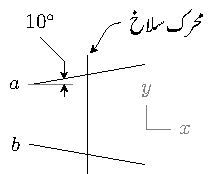
\includegraphics{figMaxwellSlidingConductorAngledRails}
\caption{محرک سلاخ پر مقناطیسی میدان محرک دباو پیدا کرتا ہے۔}
\label{شکل_میکس_ویل_سوال_محرک_سلاخ_ترچھی_ریل}
\end{figure}

جوابات:الف اور ب: \عددی{v_{ab}=-11.285t-0.08 \, \si{\volt}}، پ) \عددی{v_{ab}=-881.6t^3-t\, \si{\volt}} 
\انتہا{سوال}
%==================
\ابتدا{سوال}
رداس \عددی{\rho=\SI{0.5}{\centi\meter}} اور \عددی{\rho=\SI{4}{\centi\meter}} کی ہم محوری تار میں میدان \عددی{H_{\phi}=\tfrac{5}{\rho}\cos(2\pi\times 10^7 t - 5 z)} اور \عددی{E_{\rho}=\tfrac{8\pi^2}{\rho}\cos(2\pi \times 10^7 t -5z)} پائے جاتے ہیں۔ الف) مساوات \حوالہ{مساوات-میکس_ویل_تفرقی_الف} کے دونوں اطراف حل کرتے ہوئے ثابت کریں کہ ہم محوری تار میں موجود میدان اس پر پورا اترتے ہیں۔ ب) سمتی سطح \عددی{\phi=0}، \عددی{\SI{0.5}{\centi\meter} < \rho < \SI{4}{\centi\meter}}، \عددی{0<z<\SI{1}{\centi\meter}} اور اس کے محیط پر مساوات \حوالہ{مساوات_میکس_ویل_محرک_دباو_اور_گھٹاو_تعلق} کے دونوں اطراف حل کرتے ہوئے محرک برقی دباو حاصل کریں۔سمتی سطح کی سمت \عددی{\aphi} لیں۔یوں محیط پر چلتے ہوئے \عددی{z=\SI{1}{\centi\meter}} پر \عددی{\arho} سمت میں چلنا ہو گا۔    

جوابات:\عددی{\nabla  \times \kvec{E}=-\tfrac{\partial \kvec{B}}{\partial t}=\tfrac{40\pi^2}{\rho}\sin(2\pi \times 10^7 t - 5z)\aphi} ، \\ 
\عددی{\oint \kvec{E} \cdot \dif \kvec{L}=-\tfrac{\dif}{\dif t} \int \kvec{B} \cdot \dif \kvec{S}=52.26[\cos(2\pi \times 10^7 t -0.05)-\cos(2\pi \times 10^7 t)] \, \si{\volt}}
\انتہا{سوال}
%==================
\ابتدا{سوال}
شکل \حوالہ{شکل_میکس_ویل_سوال_کھلا_دور_بند_دور} میں \عددی{\kvec{B}=0.55\az \, \si{\tesla}} اور \عددی{\kvec{v}=6\ax\,\si{\meter\per\second}} ہیں۔محرک سلاخ میں انتہائی زیادہ مزاحمت رکھتا پیما برقی دباو \عددی{V} نسب ہے۔ الف) ساکن سلاخوں کے بائیں اور دائیں  سرے آزاد رکھتے ہوئے پیما پر کیا برقی دباو حاصل ہو گی۔ ب) ساکن سلاخوں کے بائیں سرے \عددی{a} اور \عددی{b} آپس میں موصل تار سے جوڑنے کے بعد پیما پر کیا حاصل ہو گا۔ پ) ساکن سلاخوں کے دائیں سرے آپس میں موصل تار سے جوڑنے کے بعد پیما پر کیا حاصل ہو گا۔ ت) ساکن سلاخ کے بائیں سرے آپس میں اور ان کے دائیں سرے آپس میں جوڑ کر پیما کیا پڑھے گا۔

\begin{figure}
\centering
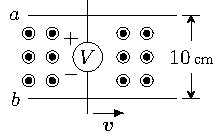
\includegraphics{figMaxwellSlidingConductorEndsOpen}
\caption{کھلے دور اور بند دور میں محرک برقی دباو۔}
\label{شکل_میکس_ویل_سوال_کھلا_دور_بند_دور}
\end{figure}

جوابات:\عددی{\SI{0}{\volt}}، \عددی{\SI{3.3}{\volt}}،  \عددی{\SI{3.3}{\volt}}، \عددی{\SI{3.3}{\volt}}
\انتہا{سوال}
%==================
\ابتدا{سوال}
برقی میدان \عددی{E=E_0 \cos 1500 t \, \si{\volt\per\meter}} کی صورت میں مندرجہ ذیل اشیاء میں ایصالی برقی رو اور انتقالی برقی رو کی شرح حاصل کریں۔ الف) تانبا جس کے مستقل \عددی{\epsilon_R=1} اور \عددی{\sigma=\SI{5.8e7}{\siemens\per\meter}} ہیں۔ ب) مقطر پانی جس کے مستقل \عددی{\epsilon_R=80} اور \عددی{\sigma=\SI{e-4}{\siemens\per\meter}} ہیں۔ پ)  کوارٹز جس کے مستقل \عددی{\epsilon_R=3.8} اور \عددی{\sigma=\SI{e-17}{\siemens\per\meter}} ہیں۔

جوابات:\عددی{\tfrac{\sigma}{\omega \epsilon}}، \عددی{4.4\times 10^{15}}، \عددی{94}، \عددی{2\times 10^{-10}}
\انتہا{سوال}
%=================

\ابتدا{سوال}
برقی میدان \عددی{E=E_0 e^{\tfrac{t}{\tau}} \, \si{\volt\per\meter}} کی صورت میں مندرجہ ذیل اشیاء میں ایصالی برقی رو اور انتقالی برقی رو کی شرح حاصل کریں جہاں \عددی{\tau=10^{-7}} کے برابر ہے۔ الف) تانبا جس کے مستقل \عددی{\epsilon_R=1} اور \عددی{\sigma=\SI{5.8e7}{\siemens\per\meter}} ہیں۔ ب) مقطر پانی جس کے مستقل \عددی{\epsilon_R=80} اور \عددی{\sigma=\SI{e-4}{\siemens\per\meter}} ہیں۔ پ)  کوارٹز جس کے مستقل \عددی{\epsilon_R=3.8} اور \عددی{\sigma=\SI{e-17}{\siemens\per\meter}} ہیں۔

جوابات:\عددی{\tfrac{\sigma \tau}{\epsilon}}، \عددی{\num{6.5e11}}، \عددی{\num{0.014}}، \عددی{\num{2.97e-11}}
\انتہا{سوال}
%=================
\ابتدا{سوال}
محدد \عددی{z} پر موجود ہم محوری تار کی لمبائی \عددی{\SI{12}{\centi\meter}} جبکہ اس کے رداس \عددی{\SI{2}{\milli\meter}} اور \عددی{\SI{6}{\milli\meter}} ہیں۔ دونوں تاروں کے درمیان مادے کے مستقل \عددی{\mu=\SI{5e-6}{\henry\per\meter}}، \عددی{\epsilon=\SI{2e-11}{\farad\per\meter}} اور \عددی{\sigma=\SI{4e-5}{\siemens\per\meter}} ہیں۔تار میں \عددی{\kvec{E}=\tfrac{10^4}{\rho}\cos (10^6t) \arho \, \si{\volt\per\meter}} کی صورت میں \عددی{\kvec{J}}، \عددی{I_c}، \عددی{\kvec{J}_d}، \عددی{I_d} اور \عددی{\tfrac{\abs{I_d}}{\abs{I_c}}} حاصل کریں۔

جوابات:\عددی{\tfrac{0.5}{\rho}\cos(10^6 t)\arho \, \si{\ampere\per\meter\squared}}، \عددی{0.12\pi\cos 10^6 t \, \si{\ampere}}، 
\عددی{-\tfrac{0.1}{\rho}\sin 10^6 t \, \si{\ampere\per\meter \squared}}، \عددی{-0.024\pi\sin 10^6 t \, \si{\ampere}}، \عددی{0.2}
\انتہا{سوال}
%==================
\ابتدا{سوال}
رداس \عددی{\rho_1} اور \عددی{\rho_2} کے ہم محوری تار کی لمبائی \عددی{l} ہے۔تار  کو بیرونی دور \عددی{V_0 \cos \omega t} برقی دباو فراہم کرتی ہے۔تار میں برقی میدان \عددی{\kvec{E}} کی مساوات لکھتے ہوئے \عددی{\kvec{J}_d} اور \عددی{I_d} حاصل کریں۔ثابت کریں کہ انتقالی برقی رو بیرونی دور میں پائی جانے والی ایصالی برقی رو کے برابر ہے۔

جوابات:\عددی{\kvec{E}=\tfrac{V_0\cos \omega t}{\rho \ln \tfrac{b}{a}}\arho \, \si{\volt\per\meter}}،
 \عددی{\kvec{J}_d=\tfrac{-\omega \epsilon V_0\sin \omega t}{\rho \ln \tfrac{b}{a}}\arho}،
  \عددی{I_d=-\tfrac{2\pi l \omega \epsilon V_0\sin \omega t}{\ln \tfrac{b}{a}}}،
 \عددی{I_c=C\tfrac{\dif V}{\dif t}=-\tfrac{2\pi l \omega \epsilon V_0\sin \omega t}{\ln \tfrac{b}{a}}}
\انتہا{سوال}
%=================
\ابتدا{سوال}
مساوات \حوالہ{مساوات-میکس_ویل_دوسری_مساوات_نقطہ_شکل_ب} کی پہلی مساوات کے دونوں اطراف پھیلاو کا عمل استعمال کرتے ہوئے  استمراری مساوات حاصل کریں۔

جواب:\عددی{\nabla \cdot \nabla \times \kvec{H}=0=\nabla \cdot \kvec{J}+\tfrac{\partial \rho_h }{\partial t}} 
\انتہا{سوال}
%====================
\ابتدا{سوال}
ایک خطہ جہاں \عددی{\kvec{E}=32\sin ax \cos 5y \cos (2\times 10^{10} t) \az} ہے کے مستقل \عددی{\mu_R=2.5}، \عددی{\epsilon_R=1.2} اور \عددی{\sigma=0} ہیں۔میکس ویل کے مساوات استعمال کرتے ہوئے \عددی{a} کی مثبت قیمت دریافت کریں۔تمام تکمل کے مستقل کو صفر لیں۔

جواب:\عددی{a=\SI{115.44}{\meter^{-1}}}
\انتہا{سوال}
%=====================
\ابتدا{سوال}
ایک ترسیلی تار میں مقناطیسی میدان \عددی{\kvec{H}=15\cos(4\times 10^9 t - \beta z) \ax \, \si{\ampere\per\meter}} پایا جاتا ہے۔ترسیلی تار کے درکار مستقل \عددی{\mu_R=1}، \عددی{\epsilon_R=5} اور \عددی{\sigma=0} ہیں۔میکس ویل کے مساوات استعمال کرتے ہوئے \عددی{\beta} کی مثبت قیمت دریافت کریں۔

جواب:\عددی{\beta=\SI{29.83}{\meter^{-1}}}
\انتہا{سوال}
%======================
\ابتدا{سوال}
موصل سطح محدد کے مرکز سے گزرتی ہے جہاں میدان \عددی{\kvec{E}=(33\ax+12\ay+25\az)\cos(10^7 t) \, \si{\volt\per\meter}} پایا جاتا ہے۔سطح کے قریب خطے کے مستقل \عددی{\sigma=0}، \عددی{\epsilon_R=12} اور \عددی{\mu_R=1.6} ہیں۔نقطہ \عددی{(0,0,0)} پر موصل سطح پہ کثافت بار حاصل کریں۔اس نقطے پر سطح کے متوازی میدان حاصل کریں۔

جوابات:\عددی{4.58\cos(10^7 t) \, \si{\nano\coulomb\per\meter\squared}}، \عددی{0}
\انتہا{سوال}
%=====================
\ابتدا{سوال}
خطہ \عددی{z<0} میں \عددی{\epsilon_{R1}=1}، \عددی{\mu_{R1}=1} اور \عددی{\sigma_1=0} ہیں جبکہ خطہ \عددی{z>0} میں \عددی{\epsilon_{R2}=9}، \عددی{\mu_{R2}=4} اور \عددی{\sigma_2=0} ہیں۔پہلے خطے میں میدان \عددی{\kvec{E}_1=[10\cos(10^9t-3.336z)-2\cos(10^9t+3.336z)]\ay} اور دوسرے خطے میں \عددی{\kvec{E}_2=(A\cos(10^9t-20.014z))\ay} ہیں۔ الف) مستقل \عددی{A} کی قیمت دریافت کریں۔ ب) مقناطیسی میدان \عددی{\kvec{H}_1} اور \عددی{\kvec{H}_2} حاصل کریں۔ پ) ثابت کریں کہ مقناطیسی میدان سرحدی شرائط پر پورا اترتے ہیں۔

جوابات:\عددی{A=8}، \عددی{\kvec{H}_1=[-0.0265\cos(10^9t-3.336z)-0.0053\cos(10^9 t +3.336z)]\ax}،\\
 \عددی{\kvec{H}_2=-0.0318\cos(10^9 t -20.014z)\ax} ،\عددی{H_{m1}=H_{m2}}
\انتہا{سوال}
%=====================
\ابتدا{سوال}\شناخت{سوال_میکس_ویل_غیر_متوقع_میدان}
خالی خلاء میں مساوات \حوالہ{مساوات_میکس_ویل_غیر_حقیقی_میدان} نلکی محدد میں میدان دیتی ہے۔خالی خلاء میں \عددی{\kvec{J}=0} لیتے ہوئے میکس ویل کی مساوات \عددی{\nabla \times \kvec{H}=\kvec{J}+\tfrac{\partial \kvec{D}}{\partial t}} استعمال کرتے ہوئے \عددی{\kvec{E}} حاصل کریں۔حاصل \عددی{\kvec{E}} سے میکس ویل کی مساوات \عددی{\nabla \times \kvec{E}=-\tfrac{\partial \kvec{B}}{\partial t}} کی مدد سے  واپس \عددی{\kvec{B}} حاصل کریں۔یوں ثابت کریں کہ دی گئی میدان میکس ویل کی مساوات پر پورا نہیں اترتا۔ 

جواب:چونکہ ہمیں واپس ابتدائی میدان حاصل نہیں ہوتا لہٰذا یہ میدان میکس ویل کی مساوات پر پورا نہیں اترتا۔
\انتہا{سوال}
%====================
\ابتدا{سوال}
دو عدد ہم محوری موصل نلکی \عددی{\rho=\SI{1}{\centi\meter}} اور  \عددی{\rho=\SI{10}{\centi\meter}} کے ساتھ سطح \عددی{z=0}  اور \عددی{z=\SI{50}{\centi\meter}} مل کر ڈبیا بناتے ہیں۔اس ڈبیا میں موجود ذو برق کے مستقل \عددی{\sigma=0}، \عددی{\epsilon_R=1.5} اور \عددی{\mu_R=2.5} ہیں جبکہ اس میں درج ذیل میدان پایا جاتا ہے۔
\begin{align*}
\kvec{H}=\tfrac{10}{\rho}\cos 2\pi z \sin (6\pi 10^7 t) \aphi \, \si{\ampere\per\meter}
\end{align*}
الف) نقطہ \عددی{N(0.01,30^{\circ},0.02)} پر سطحی کثافت برقی رو حاصل کریں۔ ب) برقی میدان \عددی{\kvec{E}} حاصل کریں۔ پ) نقطہ \عددی{N(0.015,0^{\circ},0.2)} پر سطحی کثافت بار حاصل کریں۔ ت) نقطہ \عددی{N(0.015,0^{\circ},0.2)} پر انتقالی برقی رو حاصل کریں۔

جوابات:\عددی{\kvec{K}=992\sin (6\pi 10^7 t) \, \si{\ampere\per\meter}}، \عددی{\kvec{E}=-\tfrac{25098}{\rho}\sin 2\pi z \cos(6\pi 10^7 t) \arho \, \si{\volt\per\meter}}،\\
 \عددی{\rho_S=-21.1 \cos(6\pi 10^7 t) \arho \, \si{\micro\coulomb\per\meter\squared}}، \عددی{\kvec{J}=3984\sin (6\pi 10^7 t) \arho \, \si{\ampere\per\meter\squared}}
\انتہا{سوال}
%=====================
\ابتدا{سوال}
خالی خلاء میں \عددی{V=x(z-ct) \, \si{\volt}} اور \عددی{\kvec{A}=x(\tfrac{z}{c}-t)\az \, \si{\weber\per\meter}} پائے جاتے ہیں جہاں \عددی{c=\tfrac{1}{\sqrt{\mu_0 \epsilon_0}}} کے برابر ہے۔الف ) ثابت کریں کہ \عددی{\nabla \cdot \kvec{A}=-\mu_0\epsilon_0 \tfrac{\partial V}{\partial t}} کے برابر ہے۔ ب) میدان \عددی{\kvec{B}}، \عددی{\kvec{H}} ،\عددی{\kvec{E}} اور \عددی{\kvec{D}} حاصل کریں۔ پ) ثابت کریں کہ \عددی{\kvec{J}=0} اور \عددی{\rho_h=0} کی صورت میں حاصل میدان میکس ویل کے چار مساواتوں پر پورا اترتے ہیں۔

جوابات:الف) چونکہ \عددی{\nabla \cdot \kvec{A}=x\sqrt{\mu_0 \epsilon_0}} اور \عددی{\tfrac{\partial V}{\partial t}=-\tfrac{x}{\sqrt{\mu_0 \epsilon_0}}} ہیں لہٰذا  \عددی{\nabla \cdot \kvec{A}=-\mu_0 \epsilon_0 \tfrac{\partial V}{\partial t}} ہو گا۔\\
 ب) \عددی{\kvec{B}=(t-\tfrac{z}{c})\ay \, \si{\tesla}}، \عددی{\kvec{H}=\tfrac{1}{\mu_0}(t-\tfrac{z}{c})\ay \, \si{\ampere\per\meter}}، \عددی{\kvec{E}=(ct-z) \ax \, \si{\volt\per\meter}}، \عددی{\kvec{D}=\epsilon_0 (ct-z) \ax \, \si{\volt\per\meter}}\\
 پ) حاصل میدان مساوات \حوالہ{مساوات-میکس_ویل_تفرقی_الف} تا مساوات \حوالہ{مساوات_میکس_ویل_مقناطیسی_میدان_دو_قطب} پر پورا اترتے ہیں۔ 
\انتہا{سوال}
%=================================
\ابتدا{سوال}
خالی خلاء میں دو عدد موصل چادر \عددی{y=0} اور \عددی{y=y_0} پر پائے جاتے ہیں۔ان کے درمیان درج ذیل میدان پایا جاتا ہے۔
\begin{align*}
\kvec{E}=10^4 \cos(10^7 t -6z) \ay \quad \si{\volt\per\meter}
\end{align*}
الف) \عددی{\kvec{B}} حاصل کریں۔ ب) \عددی{\kvec{A}(x,0,z,t)=0} کی صورت میں \عددی{\kvec{A}(x,y,z,t)} حاصل کریں۔ پ) \عددی{V(x,0,z,t)=0} کی صورت میں \عددی{V(x,y,z,t)} حاصل کریں۔

جواب:\عددی{\kvec{B}=-\tfrac{3}{500}\cos(10^7 t-6z) \ax \, \si{\weber\per\meter}}، \عددی{\kvec{A}(x,y,z,t)=-\tfrac{3 y}{500}\cos(10^7 t-6z) \az \, \si{\weber\per\meter}}، \\
\عددی{V(x,y,z,t)=-3.21 \times 10^8 y \cos(10^7 t -6z) \, \si{\volt}}
\انتہا{سوال}
%================================
